\documentclass[a4paper, table]{article}
% Useful packages, sorted so packages of similar functionality are grouped together. Not all are essential to make the document work, however an effort was made to make this list as minimalistic as possible. Feel free to add your own!

% Essential for making this template work are graphicx, float, tabularx, tabu, tocbibind, titlesec, fancyhdr, xcolor and tikz. 

% Not essential, but you will have to debug the document a little bit when removing them are amsmath, amsthm, amssymb, amsfonts, caption, subcaption, appendix, enumitem, hyperref and cleveref.

% inputenc, lipsum, booktabs, geometry and microtype are not required, but nice to have.

\usepackage[utf8]{inputenc} % Allows the use of some special characters
\usepackage{amsmath, amsthm, amssymb, amsfonts} % Nicer mathematical typesetting
\usepackage{lipsum} % Creates dummy text lorem ipsum to showcase typsetting 

\usepackage{graphicx} % Allows the use of \begin{figure} and \includegraphics
\usepackage{float} % Useful for specifying the location of a figure ([H] for ex.)
\usepackage{caption} % Adds additional customization for (figure) captions
\usepackage{subcaption} % Needed to create sub-figures

\usepackage{tabularx} % Adds additional customization for tables
\usepackage{tabu} % Adds additional customization for tables
\usepackage{booktabs} % For generally nicer looking tables

\usepackage[nottoc,numbib]{tocbibind} % Automatically adds bibliography to ToC
\usepackage[margin = 2.5cm]{geometry} % Allows for custom (wider) margins
\usepackage{microtype} % Slightly loosens margin restrictions for nicer spacing  
\usepackage{titlesec} % Used to create custom section and subsection titles
\usepackage{titletoc} % Used to create a custom ToC
\usepackage{appendix} % Any chapter after \appendix is given a letter as index
\usepackage{fancyhdr} % Adds customization for headers and footers
\usepackage[shortlabels]{enumitem} % Adds additional customization for itemize. 

\usepackage{hyperref} % Allows links and makes references and the ToC clickable
\usepackage[noabbrev, capitalise]{cleveref} % Easier referencing using \cref{<label>} instead of \ref{}

\usepackage{xcolor} % Predefines additional colors and allows user defined colors

\usepackage{tikz} % Useful for drawing images, used for creating the frontpage
\usetikzlibrary{positioning} % Additional library for relative positioning 
\usetikzlibrary{calc} % Additional library for calculating within tikz

% Defines a command used by tikz to calculate some coordinates for the front-page
\makeatletter
\newcommand{\gettikzxy}[3]{%
  \tikz@scan@one@point\pgfutil@firstofone#1\relax
  \edef#2{\the\pgf@x}%
  \edef#3{\the\pgf@y}%
}
\makeatother
%%%%%%%%%%%%%%%%%%%%%%%%%%%

\usepackage{parskip}
\usepackage{pdfpages} % Loads in the preamble 
% Give your report a title
\newcommand\reporttitle{Massively Learning \\Activities}
\newcommand\reporttitleheader{Massively Learning Activities}

% Insert course code, name, quartile number and year (or any other subtitle)
\newcommand\reportsubtitle{
%course code, name - Qx (2023)
}

% Add your group number (for DBL) or any other text.
\newcommand\groupnumber{
%\textbf{Group xx}
}

% Insert authors and student numbers here
\newcommand\reportauthors{
\\Master's Capstone Project\\
\\Master's of Science in Computer Science\\
\\University of Hawaii at Manoa\\\\
%Copy me & Copy me \\
}

\newcommand\reportauthorsS{
\\Under the Supervision of:\\
\\Professor Edoardo Biagioni\\
%Copy me & Copy me \\
}

% Add the name of your tutor (for DBL) or any other text.
\newcommand\grouptutor{
Tutor: %Name Surname
}

% Date and location (default: current date and Eindhoven)
\newcommand\placeanddate{
\today
}

% Define Tue-red (color of the TU/e logo). Can be changed to drastically change the look of the template
\definecolor{Tue-red}{RGB}{20, 110, 180}
\definecolor{Tue-link}{RGB}{0, 115, 187}

% All of the following code can be removed to be left with (close to) default LaTeX behaviour. 

% Sets up hyperlinks in the document to be colored
\hypersetup{
    colorlinks=true,
    linkcolor=Tue-link,
    urlcolor=Tue-link,
    citecolor = Tue-link
    }
\urlstyle{same} % Defines settings for link and reference formatting


% Change bullet style for level 1, 2 and 3 respectively for itemize
\renewcommand{\labelitemi}{\scriptsize\textcolor{Tue-red}{$\blacksquare$}}% level 1
\renewcommand{\labelitemii}{\scriptsize\textcolor{Tue-red}{$\square$}}% level 2
\renewcommand{\labelitemiii}{\textcolor{Tue-red}{$\circ$}}% level 3

% \renewcommand{\labelitemi}{\small\textcolor{Tue-red}{\ding{70}}} % level 1
% \renewcommand{\labelitemii}{\small\textcolor{Tue-red}{\ding{71}}}% level 2
% \renewcommand{\labelitemiii}{\tiny\textcolor{Tue-red}{\ding{71}}}% level 3

% Change bullet style for level 1, 2 and 3 respectively for enumerate
\renewcommand{\labelenumi}{\textbf{\textcolor{Tue-red}{\arabic*.}}}% level 1
\renewcommand{\labelenumii}{\textbf{\textcolor{Tue-red}{[\alph*]}}}% level 2
\renewcommand{\labelenumiii}{\textbf{\textcolor{Tue-red}{\roman*.}}}% level 3

% Have reference labels be linked to section (section 3 will have fig. 3.1 etc.)
\counterwithin{equation}{section} % For equations
\counterwithin{figure}{section} % For figures
\counterwithin{table}{section} % For tables

% Creates a beautiful header/footer
\pagestyle{fancy}
\lhead{TASI/PHIDC}
\rhead{\reporttitleheader}
\renewcommand{\footrulewidth}{0.4pt}
\cfoot{Page \thepage}

% Formats section, subsection and subsubsection titles respectively 
\titleformat{\section}{\sffamily\color{Tue-red}\Large\bfseries}{\thesection\enskip\color{gray}\textbar\enskip}{0cm}{} % Formats section titles

\titleformat{\subsection}{\sffamily\color{Tue-red}\large\bfseries}{\thesubsection\enskip\color{gray}\textbar\enskip}{0cm}{} % Formats subsection titles

\titleformat{\subsubsection}{\sffamily\color{Tue-red}\bfseries}{\thesubsubsection\enskip\color{gray}\textbar\enskip}{0cm}{} % Formats subsubsection titles

% Formats captions
\DeclareCaptionFont{Tue-red}{\color{Tue-red}}
\captionsetup{labelfont={Tue-red,bf}}

 % Changes font to mlmodern
%\usepackage{mlmodern}
\usepackage[sfdefault]{roboto}

% Removes indent when starting a new paragraph
\setlength\parindent{0pt}

% Limits the ToC to sections and subsections (no subsubsec.)
\setcounter{tocdepth}{2}
 % Loads in user defined settings
\begin{document}

% Inserts the front page
\begin{titlepage}

\centering

\begin{tikzpicture}

% Makes a grayed out logo as title. 
%\node[opacity=0.1,inner sep=0pt,remember picture,overlay] at (4.5,-12){
\includegraphics[width= 1.1 \textwidth]{images/TASI_logo.png}};

% Main logo on title page. 
\node[inner sep=0pt] (logo) at (0,0){
\includegraphics[width=.50\textwidth]{images/TASI_logo.png}};

% Main title, "Massively Learning Activities."
\node[text width = 1\textwidth, right = of logo](title){\sffamily\huge\reporttitle};


\node[text width = 0.5\textwidth, yshift = 0.75cm, below = of title](subtitle){\sffamily\Large \reportsubtitle};

\gettikzxy{(subtitle.south)}{\sffamily\subtitlex}{\subtitley}
\gettikzxy{(title.north)}{\titlex}{\titley}
\draw[line width=1mm, Tue-red]($(logo.east)!0.5!(title.west)$) +(0,\subtitley) -- +(0,\titley);

\end{tikzpicture}
\vspace{3cm}

\sffamily\groupnumber

\begin{table}[H]
\centering
\sffamily
\large
\begin{tabu} to 0.8\linewidth {cc}
\textbf{Full Name} & \textbf{Student ID}\\
\hline

\sffamily\reportauthors

\end{tabu}

\end{table}

%\sffamily \grouptutor

\tikz[remember picture,overlay]\node[anchor=south,inner sep=0pt] at (current page.south) {
\includegraphics[width=\paperwidth]{Figures/0. General/tue.pdf}};

\mbox{}
\vfill
\sffamily \Large \textcolor{white}{\placeanddate} \\



\end{titlepage}









\newpage

\section*{Abstract}

This paper provides an overview of UHTASI's comprehensive project with SAS technologies, which encompasses various aspects and involves partnerships with multiple agencies in the Pacific region. The project's primary objective is to establish an infrastructure for deploying SAS technologies to perform data analytics on sensitive PHI data, including healthcare claims and criminal justice records. Recognizing the urgency of the project, UHTASI has made concerted efforts to expedite the deployment of SAS technologies, focusing on their multi-tenancy capabilities and utilizing existing on-premises hardware.

Following a successful initial deployment, UHTASI plans to acquire additional hardware and migrate the existing SAS infrastructure to a new hyper-converged infrastructure (HCI) developed by UHTASI. Once the migration to HCI is complete, UHTASI aims to replicate the HCI environment and incorporate four additional tenants, enabling faculty and students at the University to access SAS technologies for research and educational purposes. Notably, the HCI instance for the University will be segregated from the original HCI, ensuring separate and secure environments.

This paper highlights the progressive steps taken by UHTASI in deploying SAS technologies, emphasizing the efficient utilization of resources and collaborative partnerships. The successful implementation of this project will contribute to improved data analytics capabilities and facilitate academic engagement with SAS technologies in the University setting.\pagenumbering{roman}
\newpage

% Generates a ToC without page number
{\hypersetup{linkcolor=black} % Keeps the ToC black even with non-black linkcolor
\renewcommand{\contentsname}{Table of Contents}
\tableofcontents\thispagestyle{empty}}
\newpage

% contains inspiration for formatting tables, images, text citations etc.
%\section{This is a section} \pagenumbering{roman}
\subsection{This is a subsection}

\subsubsection{This is a subsubsection}
This section contains some templates that can be used to create a uniform style within the document. It also shows of the overall formatting of the template, created using the predefined styles from the \texttt{settings.tex} file.

\subsection{General formaczxtting}
Firstly, the document uses the font mlmodern, using no indent for new paragraphs and commonly uses the color \textcolor{Tue-red}{Tue-red} (the color of the TU/e logo) in its formatting. It uses the \texttt{fancyhdr} package for its headers and footers, using the TU/e logo and report title as the header and the page number as the footer. The template uses custom section, subsection and subsubsection formatting making use of the \texttt{titlesec} package.\\
The \texttt{hyperref} package is responsible for highlighting and formatting references like figures and tables. For example \cref{table: style 1} or \cref{fig: three images}. It also works for citations \cite{texbook}. Note how figure numbers are numbered according to the format \texttt{<chapter number>.<figure number>}.\\

Bullet lists are also changed globally, for a maximum of 3 levels:

\begin{itemize}
    \item Item 1
    \item Item 2
    \begin{itemize}
        \item subitem 1
        \begin{itemize}
            \item subsubitem 1
            \item subsubitem 2
        \end{itemize}
    \end{itemize}
    \item Item 3
\end{itemize}

Similarly numbered lists are also changed document wide:

\begin{enumerate}
    \item Item 1
    \item Item 2
    \begin{enumerate}
        \item subitem 1
        \begin{enumerate}
            \item subsubitem 1
            \item subsubitem 2
        \end{enumerate}
    \end{enumerate}
    \item Item 3
\end{enumerate}

\newpage

\subsection{Tables and figures}
The following table, \cref{table: style 1}, shows a possible format for tables in this document. Alternatively, one can also use the black and white version of this, shown in \cref{table: style 2}. Note that caption labels are in the format \textbf{\textcolor{Tue-red}{Table x.y:} }
\begin{table}[ht]
\rowcolors{2}{Tue-red!10}{white}
\centering
\caption{A table without vertical lines.}
\begin{tabular}[t]{ccccc}
\toprule
\color{Tue-red}\textbf{Column 1}&\color{Tue-red}\textbf{Column 2}&\color{Tue-red}\textbf{Column 3}&\color{Tue-red}\textbf{Column 4}&\color{Tue-red}\textbf{Column 5}\\
\midrule
Entry 1&1&2&3&4\\
Entry 2&1&2&3&4\\
Entry 3&1&2&3&4\\
Entry 4&1&2&3&4\\
\bottomrule
\end{tabular}
\label{table: style 1}
\end{table}

\begin{table}[ht]
\rowcolors{2}{gray!10}{white}
\centering
\caption{A table without vertical lines.}
\begin{tabular}[t]{ccccc}
\toprule
\textbf{Column 1}&\textbf{Column 2}&\textbf{Column 3}&\textbf{Column 4}&\textbf{Column 5}\\
\midrule
Entry 1&1&2&3&4\\
Entry 2&1&2&3&4\\
Entry 3&1&2&3&4\\
Entry 4&1&2&3&4\\
\bottomrule
\end{tabular}
\label{table: style 2}
\end{table}

For normal, single image figures, the standard \texttt{\textbackslash begin\{figure\}} environment can be used. For multi-image figures, one could use either the \texttt{\textbackslash begin\{subfigure\}} environment to get a main caption with 3 subcaptions like \cref{fig: three images} or the \texttt{\textbackslash begin\{minipage\}} environment to get 3 independent captions like \cref{fig: style 2 image a} - \ref{fig: style 2 image c}

\begin{figure}[H]
     \centering
     \begin{subfigure}[b]{0.3\textwidth}
         \centering
         \includegraphics[width=\textwidth]{example-image-a}
         \caption{image a}
         \label{fig: style 1 image a}
     \end{subfigure}
     \hfill
     \begin{subfigure}[b]{0.3\textwidth}
         \centering
         \includegraphics[width=\textwidth]{example-image-b}
         \caption{image b}
         \label{fig: style 1 image b}
     \end{subfigure}
     \hfill
     \begin{subfigure}[b]{0.3\textwidth}
         \centering
         \includegraphics[width=\textwidth]{example-image-c}
         \caption{image c}
         \label{fig: style 1 image c}
     \end{subfigure}
        \caption{Three images}
        \label{fig: three images}
\end{figure}

\begin{figure}[H]
\centering
\begin{minipage}{0.3\textwidth}
  \centering
  \includegraphics[width=\textwidth]{example-image-a}
  \captionof{figure}{image a}
  \label{fig: style 2 image a}
\end{minipage}
\hfill
\begin{minipage}{0.3\textwidth}
  \centering
  \includegraphics[width=\textwidth]{example-image-b}
  \captionof{figure}{image b}
  \label{fig: style 2 image b}
\end{minipage}
\hfill
\begin{minipage}{0.3\textwidth}
  \centering
  \includegraphics[width=\textwidth]{example-image-c}
  \captionof{figure}{image c}
  \label{fig: style 2 image c}
\end{minipage}
\end{figure} % Feel free to remove / comment out
%\newpage

% Generates a list of symbols table
%\section*{list of symbols} \label{section: symbols}

\begin{table}[ht]
\rowcolors{2}{gray!10}{white}
\centering
\caption{list of symbols}
\begin{tabular}[t]
{m{0.1\textwidth}m{0.25\textwidth}m{0.25\textwidth}m{0.2\textwidth}}
\toprule
\textbf{Symbol}&\textbf{dimension}&\textbf{Unit}&\textbf{Unit abbreviation}\\
\midrule
1&2&3&4\\
1&2&3&4\\
1&2&3&4\\
1&2&3&4\\
\bottomrule
\end{tabular}
\end{table}
%\newpage

\pagenumbering{arabic}

% Creates the introduction, starting page numbering
\section{Introduction} \label{section: introduction}
\textcolor{red}{\lipsum[1]}
\subsection{TASI/PHIDC}

\textbf{ABOUT US}
\\
The Telecommunications and Social Informatics Research Program / Pacific Health Informatics and Data Center (TASI/PHIDC), formerly TASI/PEACESAT, is part of the Social Science Research Institute (SSRI) of the College of Social Sciences (CSS) at the University of Hawai‘i at Manoa. TASI/PHIDC programs incorporate an interdisciplinary approach to education and research, and work with partners from across the University of Hawai’i system, State of Hawai’i and other government and academic institutions from the Asia and Pacific Islands region. Program and research focus areas include policy, planning, information and communications technologies and systems, health information technology, health informatics in Hawai‘i and the Pacific Islands region.

\textbf{MISSION}
\\
The TASI/PHIDC Research Program missions are to: (1) Provide technical assistance in policy, program planning and evaluation; (2) Facilitate public and private sector collaboration to improve community resiliency, sustainability, and health system performance; and (3) Build capacity in information technology, health data management, analytics, and data sciences.

\textbf{FACULTY RESEARCH}
\\
TASI/PHIDC conducts interdisciplinary and applied research and provides policy, program, technical assistance, education, and training in Hawai‘i and the Pacific Islands Region related to:

\begin{itemize}
    \item Accessible and affordable Information and Communication Technology (ICT)
    \item Health Information Technology (HIT)
    \item Electronic Health Record (EHR)
    \item Healthcare and claims data management, analytics, and programs
    \item Telehealth
    \item Meteorological and disaster communications
\end{itemize}

\subsection{TASI \& CNMI (Contract Explained)}
TASI/PHIDC is a Technical Assistance and Research Partner or “TARP” who has an Intergovernmental Cooperative Agreement (ICA) with the Commonwealth of the Northern Mariana Islands (CNMI) State Medicaid Agency (SMA) to design an infrastructure that would allow advanced data analytics and parallel processing of Protected Health Information. After careful consideration, TASI/PHIDC has opted for SAS technologies in a hyper-converged infrastructure.

\begin{itemize}
    \item \textcolor{red}{Modernize data archive and storage (paper to electronic) of PHI data.}
    \item \textcolor{red}{Want to perform data analytics and machine learning.}
    \item \textcolor{red}{Used RCUH funds to purchase SAS license.}
    \item \textcolor{red}{Therefore, SAS needs to be accessible to multi-tenants and UH themselves.}
\end{itemize}

\subsection{TASI \& SAS (Contract Summarized)}

\begin{enumerate} 
    \item Pre-Deployment and Project Management (ETC 14 Hours)
    \begin{itemize}
        \item Before deploying SAS technologies, TASI and SAS will engage in pre-deployment and project management tasks. 
        \item These tasks will involve ongoing project management to ensure that the project plan is followed, and appropriate resources are assigned. The project plan will include details of billable work hours logs that will be sent by SAS and verified by UHTASI. In addition, SAS will send Pre-Install Requirements Documents to UHTASI for completion, and UHTASI will review the completion of these documents to ensure environmental readiness for installation. These tasks will require an estimated 14 hours of work.
    \end{itemize}
    \item Deployment (ETC 70 Hours)
    \begin{itemize}
        \item During the deployment phase, TASI will receive the installation of several SAS products:
        \begin{itemize}
            \item SAS Advanced Analytics for Education (on Viya 3.5)
            \item SAS Data Preparation
            \item SAS Data Management Advanced
            \item SAS Education Analytical Suite
            \item SAS Text Analytics for Education
        \end{itemize}
        
        \item Configuration will also be performed, which includes establishing a database connection and testing it. A validation of the new environment will be conducted to ensure that all components are working as intended before the handoff. Data libraries will be created, and SAS user access controls will be established. TASI will also verify that each of the server components is active and is handling requests. Finally, SAS will provide TASI with installation documentation.
    \end{itemize}
\end{enumerate}

\newpage

%Creates the VMware section. 
\section{VMware} \label{section: VMware}

To create a multi-tenant SAS environment, it is important to familiarize ourselves with the technology utilized by UHTASI in their existing on-premises infrastructure. UHTASI relies on VMware, a company that offers virtualization and cloud computing software solutions. Their primary software, vSphere, is used to build and manage UHTASI's on-premises infrastructure.

\subsection{vSphere 6.5}
\href{https://www.vmware.com/products/vsphere.html}{vSphere} is VMware's virtualization software suite that allows you to create and manage virtual machines and computing environments, using a set of software tools and services. With vSphere, you can run multiple virtual machines on the same physical server, each running its own operating system and applications. vSphere includes many features and capabilities that help make virtualized environments more reliable, scalable, and performant, such as: 

\begin{itemize}
    \item \textbf{ESXi}: The bare metal hypervisor installed on your machines. 
    \item \textbf{vSphere Web Client}: A web-based management interface. 
    \item \textbf{vCenter}: A centralized management system for your vSphere environment.
    \item \textbf{vSAN}: A software-defined storage solution to create a distributed storage platform in vSphere.
    \item \textbf{NSX}: A software-defined networking solution for your vSphere environment.
    \item \textbf{VMotion:} Software to migrate VMs between servers without interruption of service.
\end{itemize}

\begin{figure}[H]
    \centering
    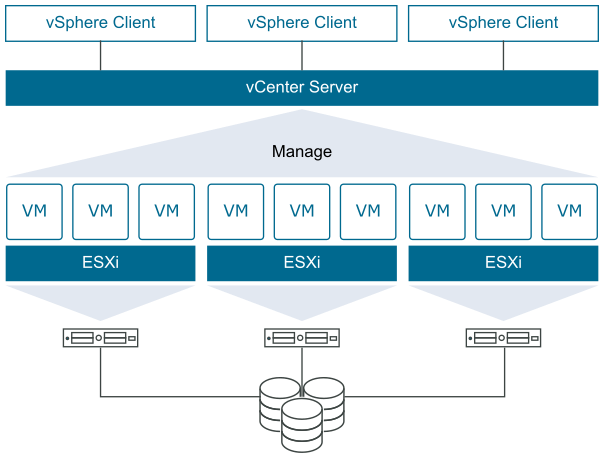
\includegraphics[scale = 0.75]{images/vmware-infrastructure-relationship.png}
    \caption{vSphere's Sotftware Suite Relationship}
    \label{VMware}
\end{figure}

\subsection{ESXi}
\href{https://www.vmware.com/products/esxi-and-esx.html}{ESXi} is a type-1, bare-metal hypervisor that is installed directly on a server and functions as the primary operating system. 

Unlike traditional operating systems (e.g., Linux, Windows Server), ESXi focuses solely on allowing virtualization. While traditional operating systems require the installation of a separate software-based type-2 hypervisor for virtualization, ESXi integrates virtualization directly into the operating system itself.

It's important to note that while ESXi enables virtualization at the OS level, the management of virtualization itself is facilitated through VMware's vSphere suite. vSphere provides the tools and features necessary to create, manage, and optimize virtualized environments. It serves as the management layer for the virtualization capabilities enabled by ESXi.

\begin{figure}[H]
    \centering
    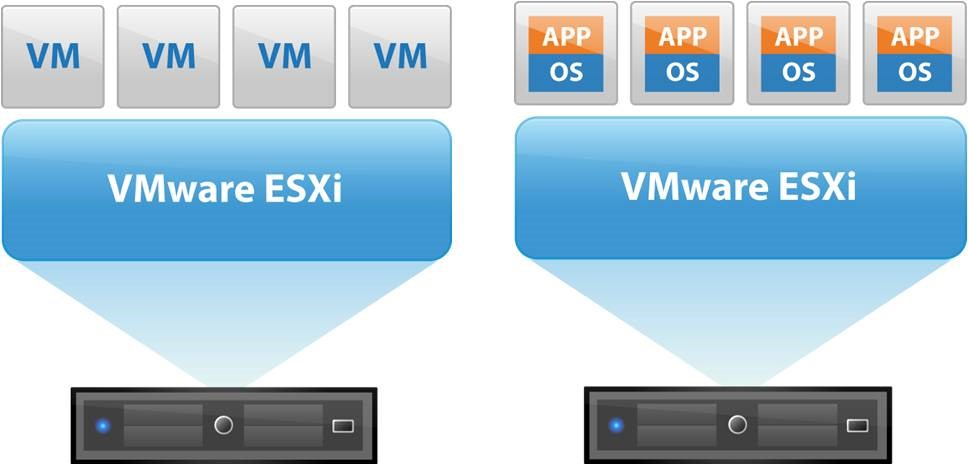
\includegraphics[scale = 0.55]{images/esxi.jpg}
    \caption{ESXi \textcolor{red}{(STOLEN EXAMPLE)} }
    \label{ESXi}
\end{figure}

\subsection{vSphere Client}
The \href{https://docs.vmware.com/en/VMware-vSphere/7.0/com.vmware.vsphere.vcenterhost.doc/GUID-A618EF76-638A-49DA-991D-B93C5AC0E2B1.html}{vSphere Client} is an application (interface) that allows you to manage and monitor your VMware environments. It is important to note that the actual management capabilities stem from the vCenter Server and \textbf{NOT} from vSphere client.

\begin{figure}[H]
    \centering
    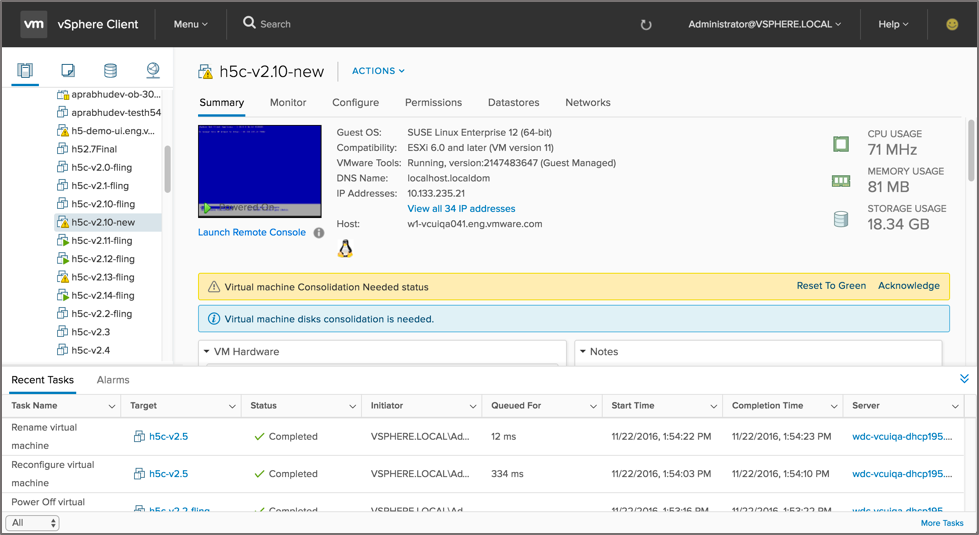
\includegraphics[scale = 0.9]{images/vsphere-client.jpg}
    \caption{vSphere Client \textcolor{red}{(STOLEN EXAMPLE)} }
    \label{vSphere Client}
\end{figure}

\subsection{vCenter}
The vCenter Server is a centralized platform for managing vSphere environments. 

While vSphere serves as the foundation for virtualization, vCenter Server extends these capabilities by acting as a centralized platform designed to manage vSphere environments. Beyond the basic management features offered by vSphere, vCenter Server offers advanced functionalities such as automation, orchestration, and policy-based management.

Some key features of vCenter include: VM migration, security groups, role policies, single sign-on, workflow automation, monitoring and auditing reports, distributed resource management, and optimized resource allocation.

\subsubsection{vCenter Security and Risks}
Security is a critical aspect of virtualized environments, and vCenter provides a range of security features to protect against unauthorized access, data theft, and data manipulation. These security features include: role-based access control\footnote{Define roles and permissions to users based on their roles to prevent unauthorized access.}, auditing\footnote{Track user activity and changes to identify security issues and log actions taken within the virtualized environment.}, encryption\footnote{Encrypt VM data, configuration files, and communication between hosts.}, secure communication\footnote{Supports SSL/TLS encryption to secure communication between hosts and the vCenter server.}, integration\footnote{Integrate with third-party security products (e.g., antivirus, IDS) to provide additional layers of security}, and two-factor authentication\footnote{Provide two forms of identification before accessing the VM to prevent unauthorized access.}. These security features help to ensure confidentiality, integrity, and availability of the virtualized infrastructure, a requirement when working with PHI data. 

\subsection{vSAN}
\href{https://docs.vmware.com/en/VMware-vSphere/7.0/com.vmware.vsphere.vsan-planning.doc/GUID-A80526C8-A941-4F84-9D44-D4B8B3914A95.html}{vSAN} is a software-defined storage solution developed by VMware, which allows organizations to create a distributed storage platform that is integrated with vSphere. This provides a highly scalable and available storage infrastructure, using standard hardware.

By creating a shared data store using the internal disks of ESXi hosts in a vSphere cluster, vSAN allows organizations to pool their storage capacity and performance into a single datastore, scaling it easily by adding more hosts to the cluster. vSAN features data replication, erasure coding, and automatic data rebalancing. Additionally, it offers advanced storage services such as deduplication, compression, and encryption, ensuring optimal storage efficiency and security which streamlines storage management, automates routine tasks, and helps to optimize storage utilization and cost savings.

\begin{figure}[H]
    \centering
    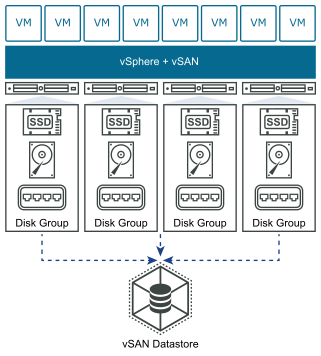
\includegraphics[scale = .8]{images/vsan-deployment.png}
    \caption{Standard vSAN Cluster \textcolor{red}{(STOLEN EXAMPLE)} }
    \label{vSan}
\end{figure}

\subsection{NSX}
\href{https://docs.vmware.com/en/VMware-NSX/index.html}{NSX} is a network virtualization and security platform created by VMware that provides a software-defined networking (SDN) solution that enables organizations to virtualize their network infrastructure, creating a more flexible, scalable, and manageable network.

NSX allows for all network components in your infrastructure to be virtualized, decoupling your network from existing hardware. This abstraction enables organizations to pool and automate network resources, which can reduce the time and cost of deploying and managing network infrastructure. NSX also offers advanced security features and networking capabilities which allows administrators to apply precise policies to specific workloads or applications. For example, NSX provides: network automation, multi-cloud and on-premises support, network segmentation, minimal cost and resource overhead, switching and routing, and load balancing features. 

\begin{figure}[H]
    \centering
    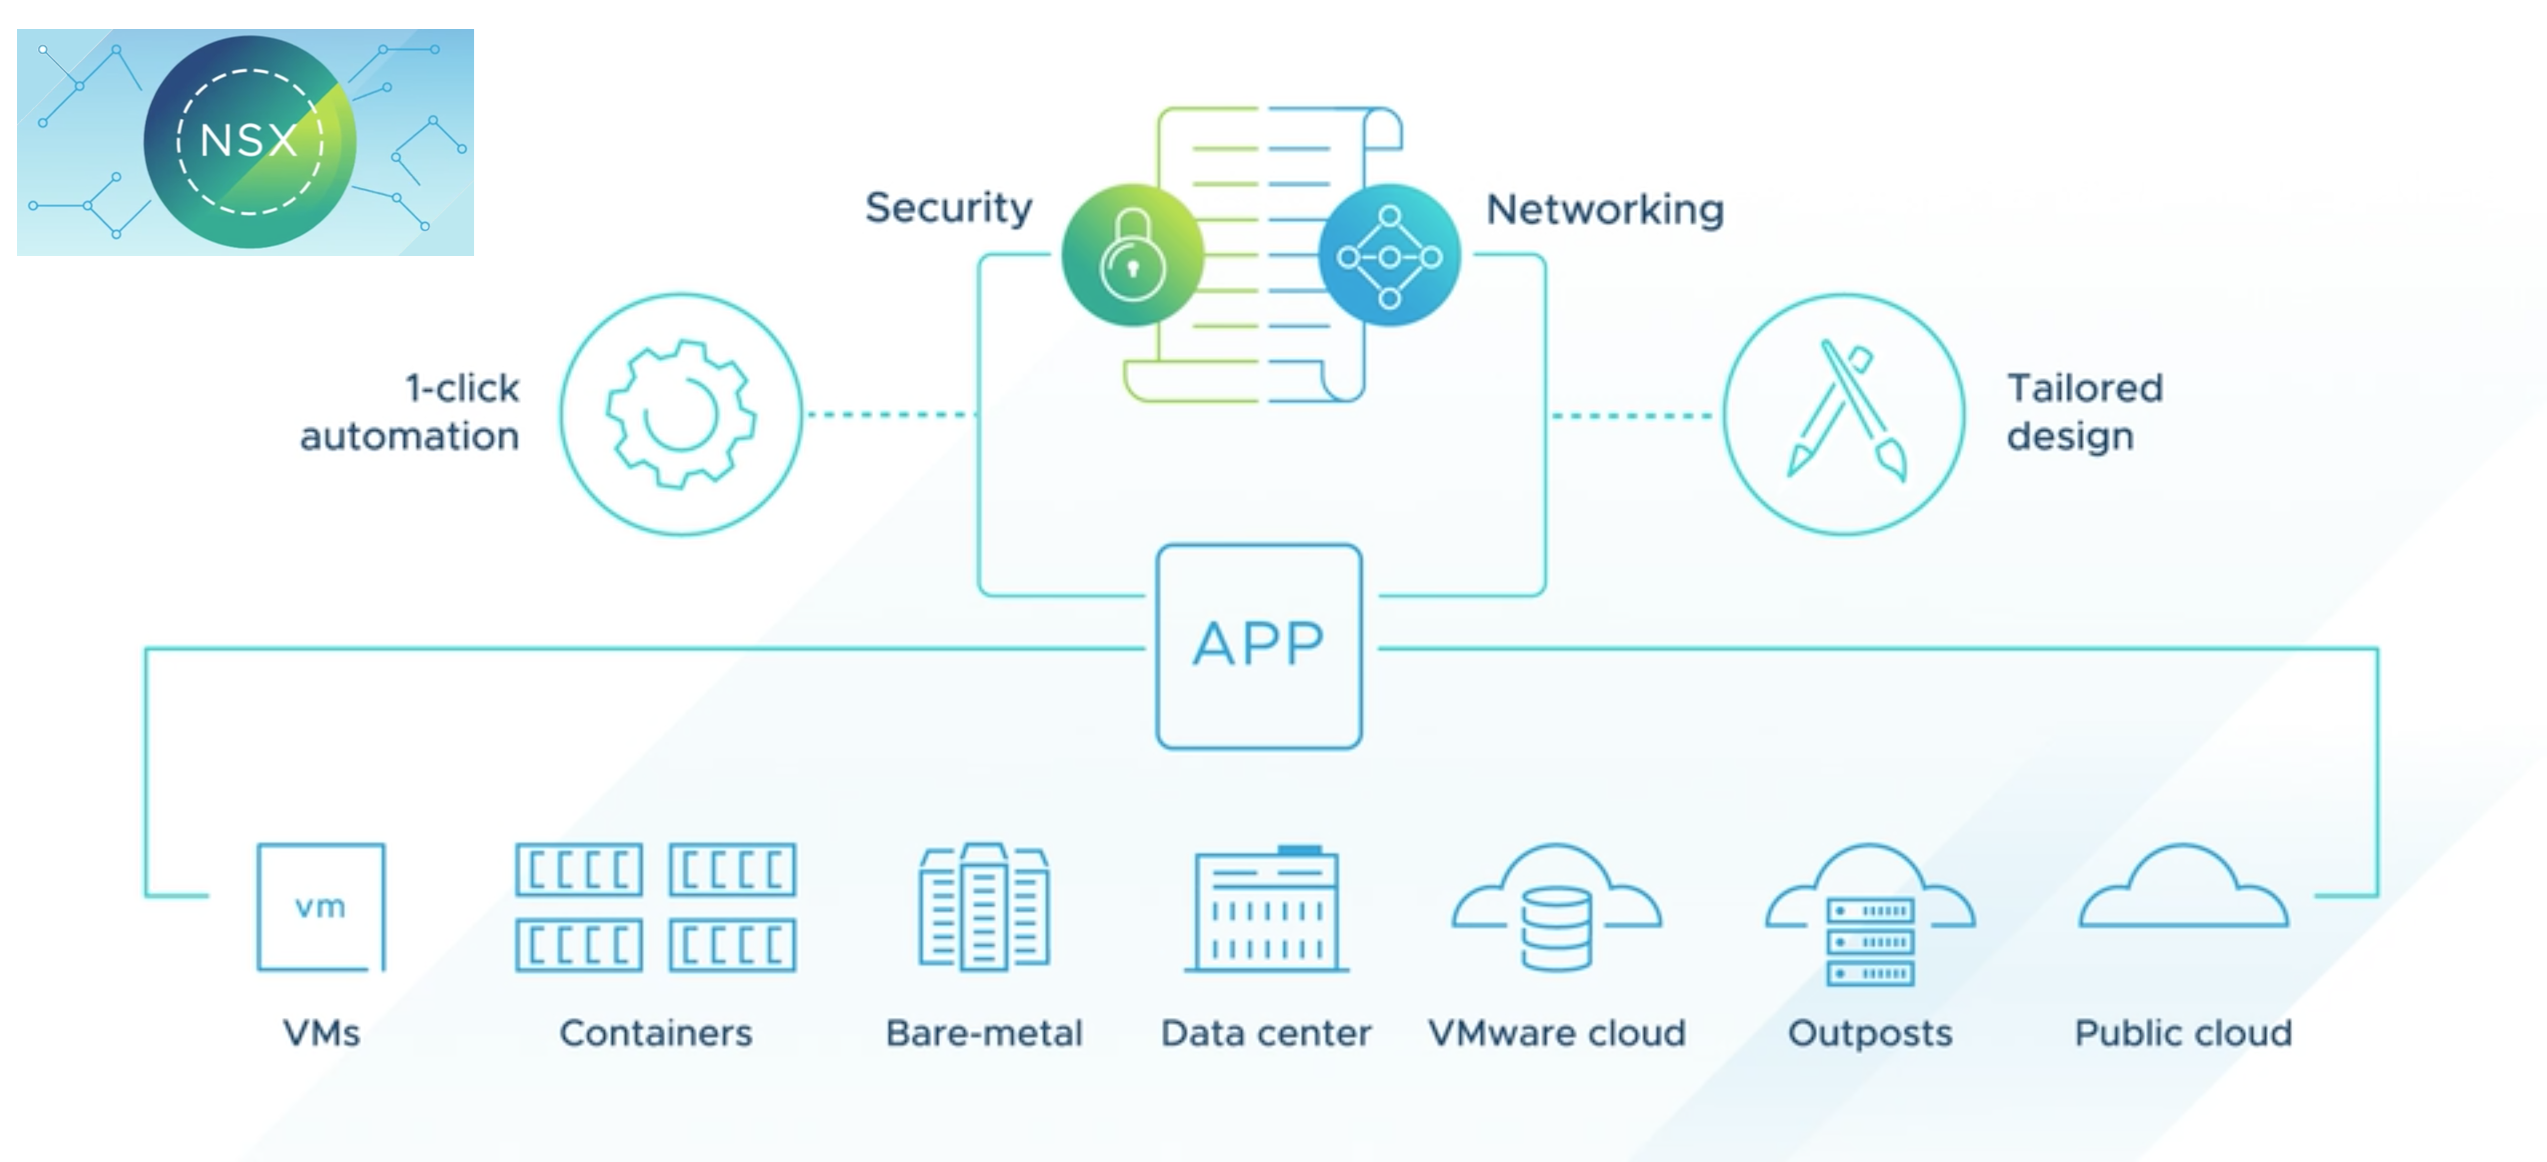
\includegraphics[scale = .19]{images/nsx-diagram.png}
    \caption{NSX Infrastructure \textcolor{red}{(STOLEN EXAMPLE)} }
    \label{NSX}
\end{figure}

\subsection{VMotion}
\href{https://www.vmware.com/products/vsphere/vmotion.html#:~:text=vMotion%20allows%20you%20to%3A,a%20virtual%20machine%20in%20seconds}{VMotion} is virtualization software that enables IT administrators to move VMs between physical servers or hosts without disrupting service. The process involves copying the entire state of the VM, including memory, CPU state, and network connections, from one host to another. The benefits of VMotion include increased availability and uptime, improved hardware utilization, workload balancing, and reduced downtime for maintenance and upgrades. However, the feature also requires specialized hardware and software, increasing the complexity of virtualized environments. VMotion uses shared storage, high-speed networking, and specialized software to ensure a seamless migration. 

The main use case for VMotion is to provide high availability and workload balancing for virtualized environments by optimizing resource usage, improving performance, and avoiding downtime during maintenance or upgrades. For example, an IT administrator can use VMotion to move running VMs to another host during server maintenance, ensuring uninterrupted service for end-users. Once the maintenance is complete, the VMs can be moved back to the original host. VMotion also allows for the consolidation of workloads and the migration of VMs to new hosts for improved hardware utilization and cost savings.

When migrating VMs with sensitive data, such as protected health information (PHI), there may be compliance issues with regulations like HIPAA. To ensure compliance, virtualization infrastructure and VMotion must be configured to meet data protection, access control, and auditability requirements. Encryption and other security measures should also be implemented to protect the confidentiality, integrity, and availability of PHI during migration. IT administrators should ensure that host servers and network connections used for VMotion are secure and protected from unauthorized access.

\begin{figure}[H]
    \centering
    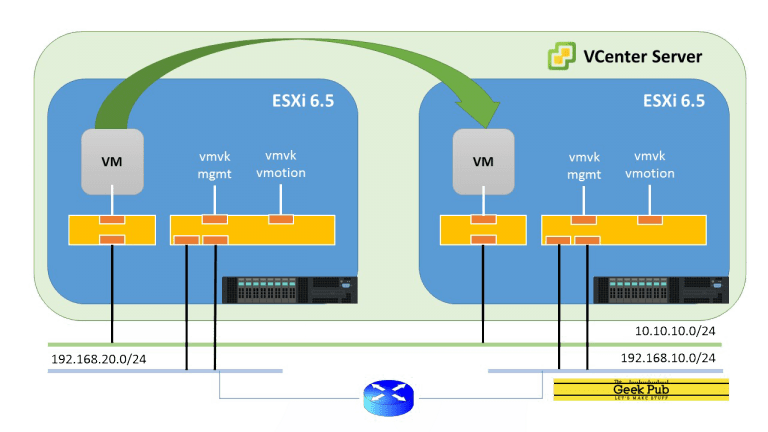
\includegraphics[scale = .50]{images/vmotion.png}
    \caption{VMotion \textcolor{red}{(STOLEN EXAMPLE)} }
    \label{VMotion}
\end{figure}
\newpage

%Creates the SAS section.
\section{Statistical Analysis System (SAS)} \label{section: SAS}
SAS, or Statistical Analysis System, is a software suite that has been used for advanced analytics, business intelligence, data management, and predictive analytics since it was first released in 1976. Developed by the SAS Institute, it offers a range of statistical and data analysis tools, which are suitable for many applications including data mining, forecasting, econometrics, quality control, and statistical analysis.

The software provides a user-friendly graphical interface for data analysis and reporting, as well as a powerful programming language that allows users to customize their analysis and automate repetitive tasks. Its ability to handle large and complex datasets and perform advanced statistical analyses make it popular in various industries, including finance, healthcare, government, and academia. SAS is widely used for purposes such as fraud detection, risk management, clinical research, and marketing analysis, and is a popular choice among data scientists and statisticians. 

SAS offers multiple product\href{https://www.sas.com/en_us/software/all-products.html#all-products-a-z}{\textbf{ suites}}. The SAS Enterprise Suite is a collection of SAS products designed for enterprise-level data management and analysis. The SAS Platform provides two engines for managing foundational capabilities such as distributed processing, security, administration, program development and execution, resource management, user interfaces, cloud integration, operating systems and third-party software. These engines are SAS 9.4 and SAS Visual Analytics. 

In addition to the SAS Enterprise Suite and the SAS Platform, SAS also offers SAS Data Management Advanced which is a powerful ETL solution for preparing data for both analytic engines.

\subsection{SAS Data Management Advanced (SAS DMA)}
SAS Data Management Advanced (SAS DMA), is a software suite that provides a comprehensive set of tools for data integration and data quality. The primary purpose of SAS DMA is to support data ETL (Extract, Transform, Load) processes, which involve extracting data from multiple sources, transforming it to meet specific requirements, and loading it into a target system for analysis and reporting. SAS DMA is a stand-alone software suite and can be deployed on-premises or in the cloud. It is not part of SAS 9.4 (i.e. SAS Data Management and Analytics), which is a separate software suite that provides a wide range of tools for data analysis, reporting, and visualization.

To support these functions, SAS DMA relies on three different types of servers:

\begin{itemize}
    \item The \textbf{Mid-Tier} server is a web-based interface that provides access to SAS DMA workflows. This server is responsible for user authentication and authorization, job scheduling and monitoring, and other functions that are necessary for effective workflow management. It acts as a gateway for users to interact with the SAS DMA system.
    \item The \textbf{Metadata} server is responsible for managing information about data sources and workflows. It provides a central repository for storing metadata, which enables efficient management of SAS objects, definition of relationships between objects, and tracking of changes to data. In the case of SAS DMA, the metadata server manages information about data integration workflows and data quality rules.
    \item The \textbf{Compute} server provides the processing power and resources necessary to run data integration and data quality jobs. This server is responsible for executing the actual data integration and ETL tasks defined in the workflows created in SAS DMA. It ensures that the workflows are run efficiently and effectively, regardless of the size or complexity of the data being processed.
\end{itemize}

\subsection{SAS 9.4}
\href{https://documentation.sas.com/doc/en/pgmsascdc/9.4_3.5/whatsnew/n17cszme3e52b4n1ooe3710fnuec.htm#:~:text=For%20SAS%20administrators%2C%20SAS%209.4,more%20complete%20data%20management%20solution.}{SAS 9.4} is a software suite that provides tools for data management, statistical analysis, business intelligence, and predictive modeling. SAS 9.4 can handle large datasets and complex analyses by using a wide range of built-in functions and procedures that can save time and effort when working with data. 

For example, a pharmaceutical company might use SAS 9.4 to analyze clinical trial data to determine the efficacy and safety of a new drug. A bank might use SAS 9.4 to perform risk analysis on its loan portfolio. A retail company might use SAS 9.4 to analyze customer data to better understand buying patterns and preferences.

SAS 9.4 is composed of several modules that provide a wide range of functionalities:
\begin{itemize}
    \item Base SAS - The basic programming language, data access, and management capabilities of SAS.
    \item SAS/STAT - A comprehensive set of statistical analysis procedures for data exploration and modeling.
    \item SAS/GRAPH - A set of tools for creating high-quality graphical output from SAS data.
    \item SAS/ETS - A set of time series analysis and forecasting procedures.
    \item SAS/IML - An interactive matrix language for matrix manipulation, data analysis, and numerical optimization.
    \item SAS/ACCESS - Connectivity to data sources such as relational databases and spreadsheets.
    \item SAS Enterprise Guide - A graphical user interface (GUI) for SAS programming, data management, and reporting.
\end{itemize}

\subsection{SAS Visual Analytics (SAS Viya)}
SAS Visual Analytics (\href{https://documentation.sas.com/doc/en/pgmsascdc/9.4_3.5/pgmsasgswlcm/home.htm}{SAS Viya}), is a cloud-based analytics platform that provides a suite of tools and services for elastic, scalable, and fault-tolerant data analytics, data processing, and machine learning for enterprise environments. It allows organizations to store, manage, analyze, and share large volumes of data across different sources and formats, all within a single platform. 

SAS Viya is composed of several software that provide a wide range of functionalities:

\begin{itemize}
    \item SAS Visual Analytics: A tool for creating interactive reports and dashboards to explore and visualize data.
    \item SAS Visual Statistics: A tool for performing statistical analysis and building predictive models on large data sets.
    \item SAS Visual Data Mining and Machine Learning: A tool for exploring and analyzing large data sets using advanced analytics techniques such as clustering, decision trees, and neural networks.
    \item SAS Visual Forecasting: A tool for creating accurate and reliable forecasts using time series data.
    \item SAS In-Memory Statistics: A tool for performing high-performance analytics and modeling on large data sets using in-memory processing.
\end{itemize}

When performing analytics on large datasets, SAS Viya uses Cloud Analytic Services.

\subsection{Cloud Analytics Services (CAS)}
Cloud Analytics Services (\href{https://documentation.sas.com/doc/en/calcdc/3.3/calserverscas/n05000viyaservers000000admin.htm}{CAS}) is the in-memory analytics engine SAS Viya uses for both on-premise as well as cloud-service environments (e.g., AWS, Azure, GCP). CAS uses a combination of hardware and software where data management and analytics take place on either a single-machine or as a distributed server across multiple machines. In either single or distributed deployment, each machine (host, node, etc) will be assigned one of three roles: CAS Controller, CAS Backup Controller, CAS Worker.

\textbf{Analogy}
\\
In a restaurant kitchen, there exists three primary chefs. They are the (1) executive chef, (2) sous chef, and (3) station chef(s). The executive chef's primary role is to manage the kitchen and its staff whilst doing very little cooking. The sous chef's primary role is to be the right-hand to the executive chef, ready to manage the kitchen, share, or take over the responsibility of the executive chef at a moments notice. The station chef(s) merely wait for instructions from the executive chef, then executes the job they are given. 

This is the relationship of each CAS node with each other:
\begin{itemize}
    \item The CAS Controller is the executive chef managing the kitchen and its staff, delegating work.
    \item The CAS Backup Controller is the sous chef ready to take over the responsibility of the executive chef. 
    \item The CAS Worker(s) are the station chefs cooking what they are assigned to by the executive chef. 
\end{itemize}

\subsubsection{Role 1: CAS Controller}
Controller is the first role that can be assigned to a host for SAS Cloud Analytic Services. For both server architectures, single-machine and distributed, one machine must be designated as the Controller. The role of the Controller is to parse out work to each Worker host available. In other words, the Controller manages and controls the overall operation of the CAS environment. As the master node, the Controller is responsible for distributing workload among available CAS Workers, managing user sessions, and providing a secure environment for data retrieval and data storage. 

In a single-machine environment, the CAS Controller and CAS Worker roles can be performed by different processes or threads within the same operating system instance. However, we are not limited to this deployment method as it is also possible to have the CAS Controller and CAS Worker(s) virtually separated (on the same hardware) to increase the scalability of the deployment. The configuration of your architecture depends on what you need out of CAS.  

In a distributed environment, the CAS Controller is responsible for managing and controlling the CAS environment whilst the actual data processing and data analytics are performed by the CAS Worker(s).
%insert diagram%

\subsubsection{Role 2: CAS Backup Controller}
Backup Controller is the second role that can be assigned to a host for SAS Cloud Analytic Services. Although optional, the CAS Backup Controller is highly recommended in a distributed server environment. The role of the CAS Backup Controller is to act as a standby or hot-backup for the primary CAS Controller in case of a failure. Its primary purpose is to ensure that the system can continue to function in the event of a failure of the primary controller. The Backup Controller is typically set to passively monitor the primary controller for any signs of failure, such as a loss of connectivity or failure to respond to heartbeat messages. It does not actively participate in task scheduling or job execution while the primary controller is running normally. 

If the primary CAS Controller fails, the Backup Controller will take over as the primary controller and assume responsibility for managing the CAS worker nodes and scheduling tasks. In this scenario, the CAS worker nodes will send their status updates and job results to the Backup Controller instead of the failed primary controller.\footnote{If the main CAS Controller fails, how does each CAS Worker respond to the Backup Controller with their completed jobs?}

In some systems, the Backup Controller can also be given jobs to execute as a CAS worker node. This can help to improve the system's overall performance by increasing the number of available processing resources. In this scenario, the Backup Controller can perform both the role of a CAS Controller and a CAS worker node.\footnote{Can the CAS Backup Controller be assigned work as well as passively monitor the main CAS Controller?}

%insert diagram%

\subsubsection{Role 3: CAS Workers}
Worker is the third role that can be assigned to a host for SAS Cloud Analytic Services. The CAS Worker is responsible for performing data processes and data analytics sent from the CAS Controller. For example, CAS Workers can perform data manipulations, transformations or computations on large/complex datasets. These computations are but not limited to: statistical analysis, machine learning models, text analysis, time series analysis, optimization, etc. Workers execute these computations using data stored on disk, in-memory, or in a distributed file system. 

In a distributed environment, one host will be assigned as your controller and any additional hosts are considered workers (optional CAS Backup Controller). Workers increase the overall computing power of your distributed-server and provides a solution for a scalable (up/down), distributed, and fault-tolerant environment for data storage and data analysis because the worker manages the storage of data/metadata across multiple nodes. The amount of CAS Workers needed to create an optimized distributed environment is highly dependant on data size, computation type, and workload.  
%insert diagram%

We can create two types of CAS configurations: a single-machine environment using symmetric multiprocessing \href{https://documentation.sas.com/doc/en/calcdc/3.3/calserverscas/n05000viyaservers000000admin.htm}{\textbf{(SMP)}}, or distributed server environment using massively parallel processing \href{https://documentation.sas.com/doc/en/calcdc/3.3/calserverscas/n05000viyaservers000000admin.htm}{\textbf{{(MPP)}}}.

\subsubsection{Symmetric Multiprocessing (SMP)}
The Symmetric multiprocessing (SMP) architecture is used when you want to run CAS on a single server or virtual machine (VM) with multiple CPU cores. This is called shared-memory architecture because all the CPUs share the same memory. When a job is submitted to CAS in an SMP architecture, it is processed by the worker node(s) in parallel using the shared memory. The results are returned to the controller node, which sends them back to the user.

A typical SMP architecture for CAS might consist of a single VM that serves as both the controller and worker node. The number of VMs required will depend on the size of your data and the processing requirements of your workload. For example, if you have a large dataset or complex analytical workloads, you might deploy CAS on a VM with 8 or 16 CPU cores.

Some examples of use cases for CAS on an SMP architecture include:

\begin{itemize}
    \item Exploratory data analysis
    \item Statistical modeling and regression analysis
    \item Predictive analytics
    \item Machine learning and deep learning
\end{itemize}

\begin{figure}[H]
    \centering
    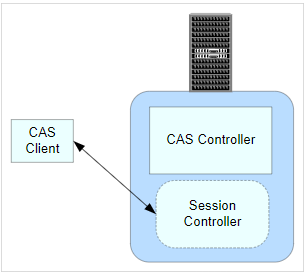
\includegraphics[scale = 0.8]{images/smp_server.png}
    \caption{Single-machine CAS Server \textcolor{red}{(STOLEN EXAMPLE)} }
    \label{SMP Achitecture}
\end{figure}

\subsubsection{Massively Parallel Processing (MPP)}
The Massively Parallel Processing (MPP) architecture is used when you want to run CAS on a cluster of multiple servers or VMs. This is called distributed-memory architecture because the data is partitioned and stored across multiple servers or nodes. When a job is submitted to CAS in an MPP architecture, it is distributed across the worker nodes in parallel. Each worker node processes its own subset of the data and returns the results to the controller node. The controller node then aggregates the results from all worker nodes and sends them back to the user.

A typical MPP architecture for CAS might consist of multiple VMs or servers, with some dedicated as controller nodes and others as worker nodes. The number of VMs or servers required will depend on the size of your data and the processing requirements of your workload. For example, you might choose to deploy CAS on a cluster of 10 or more VMs or servers to handle large-scale data processing tasks.

Some examples of use cases for CAS on an MPP architecture include:
\begin{itemize}
    \item Big data processing and analysis
    \item High-performance computing
    \item Large-scale machine learning and deep learning
    \item High-throughput data processing, such as in genomics or drug discovery
\end{itemize}

\begin{figure}[H]
    \centering
    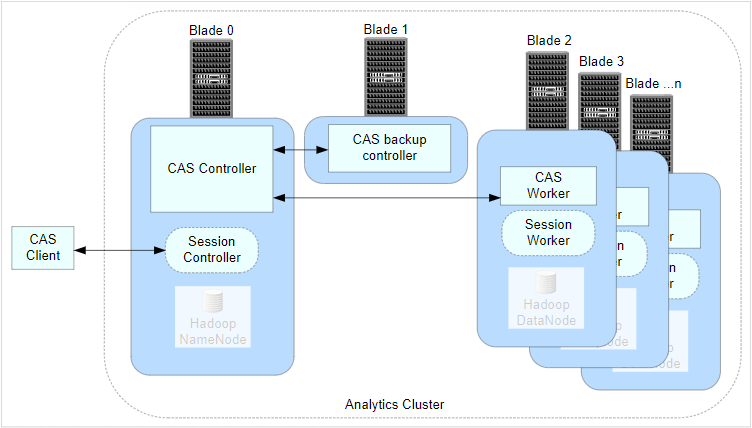
\includegraphics[scale = 0.70]{images/mpp_server.png}
    \caption{Distributed CAS Server \textcolor{red}{(STOLEN EXAMPLE)} }
    \label{MMP Architecture}
\end{figure}


\newpage

%Creates the Massively Learning Activities section.
\section{Security and Risk Management} \label{section: SARM}
This chapter provides an introduction to security and risk management by covering key concepts such as data compliance, identity and access management (IAM), data governance, data encryption, and data backups. This chapter is not intended to be a comprehensive handbook for implementing proper security measures, but rather as an overview of the security measures to consider when developing a strategy for storing and accessing sensitive information.

\subsection{Data Compliance}

\begin{itemize}
    \item HIPAA Compliance
    \item UHM Compliance
    \item RCUH Compliance
    \item TASI Compliance
    \item State of Hawaii Compliance
\end{itemize}

\subsection{Identity and Access Management (IAM)}
Identity and Access Management (IAM) is a security practice that safeguards sensitive information by allowing only authorized individuals to access confidential resources and data. 

Identity management looks to confirm that an accessing user is who they say they are, whilst access management uses a users identity to determine which resource they are allowed to access. 

IAM components can be classified into four major categories: authentication, authorisation, user management, and central user repository.

\subsubsection{Authentication}
Authentication is a component of IAM in which a user is required to provide sufficient credentials to gain access to an application system. 

Sufficient credentials for accessing sensitive healthcare information are defined as authentication methods that comply with the HIPAA Security Rule (Section 5.1). The HIPAA Security Rule requires covered entities to implement multi-factor authentication or an equivalent authentication method for accessing ePHI.

According to HIPAA, the multi-factor authentication method must use two of the following three elements:

\begin{itemize}
    \item Something you know (Password or PIN)
    \item Something you have (Smart Card or Security Token) 
    \item Something you are  (Fingerprint or Facial Recognition)
\end{itemize}

Two new additional standards are not required but provide additional authentication methods:

\begin{itemize}
    \item Somewhere you are (IP Address or Geo-location)
    \item Something you do (Signature or Gesture)
\end{itemize}

Once a user is authenticated, a session is created to allow the user to interact with the application system. The session will remain open until the user's task is completed or through termination by other means (e.g., timeout). By centrally maintaining the session of a user, the authentication module can provide single sign-on services. 

Single sign-on (SSO) is a mechanism that allows users to authenticate once and access multiple systems or applications without having to re-enter their credentials. SSO simplifies access control and user permissions by providing a centrally managed solution for user authentication policies across all systems. There are several options when deciding on a SSO solution. (e.g., LDAP, OAuth, SAML, RADIUS, PKI, etc).

\subsubsection{Authorization}
Authorization is a component of IAM in which a user is given permission to access a particular resource. 

This component comes after a user has successfully authenticated to an application system with sufficient credentials. Authorization is performed by checking the resource access request (e.g., web-based application URL), against an IAM policy store and is the core module that implements Role-Based/Attribute-based, access control. 

\begin{itemize}
    \item Role-Based Access Control (RBAC) is a method of access control that assigns roles to users  and access permissions to those roles in order to provide a centrally managed solution for authorization. 
    \item Attribute-Based Access Control (ABAC) is a method of access control that assigns permissions based on a user's attributes (e.g., job title, location, department). 
\end{itemize}

The authorization model can provide more complex access control policies other than user role/groups and user attributes (e.g., access channels, time, resource requested, external data, business rules). 

\subsubsection{Central User Repository}
The Central User Repository (CUR) stores and delivers identity information in order to verify credentials submitted from clients. Identity information is equivalent to user account information (e.g., usernames, passwords, etc). The most common CUR protocol is the Lightweight Directory Access Protocol (LDAP). 

LDAP is a protocol for accessing and maintaining distributed directory information services over an Internet Protocol network in order to provide a centrally managed authentication and authorization solution for application systems. 

LDAP allows system administrators to manage user accounts, configure access and permissions, and monitor and audit user activity.

\begin{figure}[H]
    \centering
    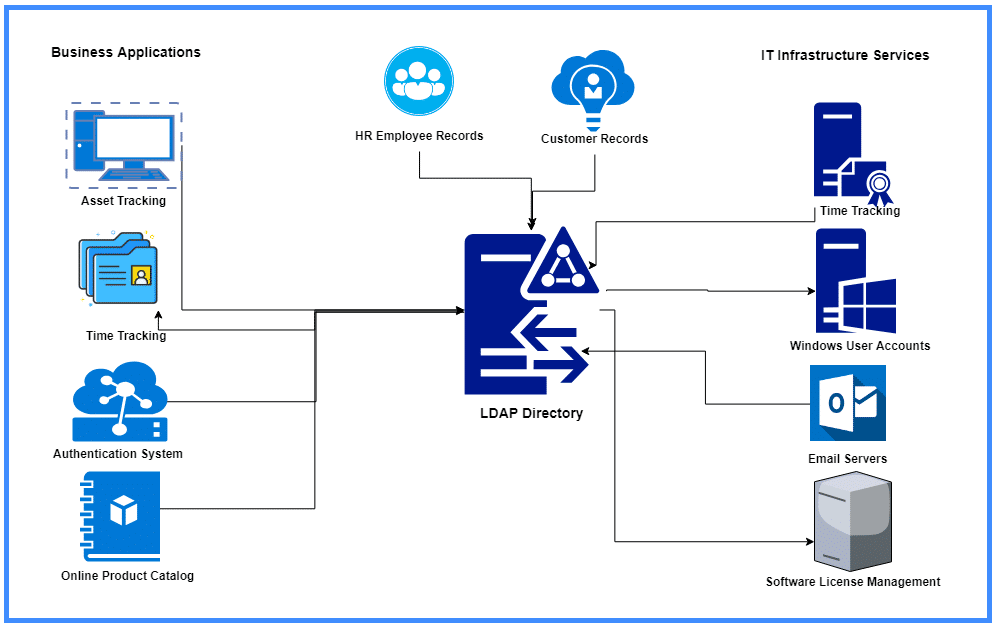
\includegraphics[scale = 0.6]{images/LDAP.png}
    \caption{Lightweight Directory Access Protocol \textcolor{red}{(STOLEN EXAMPLE)} }
    \label{LDAP}
\end{figure}

When designing an LDAP directory, it is important to consider the principle of least privilege. The principle of least privilege is a design principle where each user or service is only given the necessary permissions to perform their intended tasks, and no more. Unauthorized users should not access important data or systems. The principle of least privilege should also be considered when designing security groups and access control lists, as unauthorized users must not have access to sensitive information.

\subsubsection{User Management}

User Management is the component of IAM that covers the creation and maintenance of user accounts, account identity, and account privileges. 

Identity creation and maintenance is controlled by the set of administrative functions such as user life-cycle management, role/group management, and user/group provisioning. User life-cycle management controls the lifespan of user accounts from account provision to account deprovision. Role/group management and user/group management is used for user authorization (Section 5.2.2). 

Onboarding, maintenance, and off-boarding are the three components of user life-cycle management. 

\begin{enumerate}
    \item On-boarding Process:
        \begin{itemize}
            \item Account authentication for relevant systems and applications.
            \item Verification of tenant identity.
            \item Setting up multi-factor authentication.
            \item Domain and network access configuration.
            \item Training for new tenants on how to use the systems and applications they have access to.
        \end{itemize}
    \item Maintenance Process:
        \begin{itemize}
            \item Regular review of tenant access privileges to ensure that they align with the tenant's job function and level of responsibility.
            \item Management of access requests and approvals to ensure that access is only granted to authorized tenants.
            \item Management of tenant accounts and passwords, including password expiration policies and periodic password resets.
            \item Monitoring and auditing tenant activity to detect for potential security threats.
            \item Provisioning of additional access or permissions based on changes to the tenant's role or job function.
        \end{itemize}
    \item Off-boarding Process:
        \begin{itemize}
            \item Revocation of tenant access to all systems and applications once life-cycle is expired. 
            \item Archiving or removal of tenant data in accordance with the organizations (e.g., TASI, RCUH, UHM, etc.) policies and regulatory requirements.
            \item Review of tenant access to ensure that no data or resources have been left behind.
            \item Disabling or revocation of any credentials associated with the tenant's access.
            \item Notification of relevant stakeholders about the tenant's departure.
        \end{itemize}
\end{enumerate}

\subsection{Data Governance}
\textcolor{red}{\textbf{To be completed during the Data Governance Seminar in early May 22-24, 2023.}}

\subsection{Data Encryption}

Data Encryption is a security practice that safeguards sensitive information by transforming the data into an unreadable format that can only be deciphered with the appropriate decryption key. 

HIPAA Security Rule (Section 5.1) requires covered entities to implement a mechanism to encrypt and decrypt ePHI based on the assessment of risks to the confidentiality, integrity, and availability of the ePHI. 

\begin{itemize}
    \item Data At-Rest is data that is stored in storage devices (e.g., disk, tap, USB drives, non-votalite storage, etc) and is not being used or transmitted.
    \item Data In-Transit is data that is transmitted over a network (e.g., file transfers, emails, instant messages). HIPAA requires the use of secure transmission protocols (e.g., SSL, TLS) for transmitting ePHI over public networks. 
\end{itemize}

\subsection{Data Backup}

A Data Backup is a copy of data that is used for data restoration in the case of data loss, data corruption, or other data-related disasters.

\begin{itemize}
    \item Recovery Point Objective (RPO) is the maximum amount of data – as measured by time – that can be lost before data loss exceeds what is acceptable to an organization.
    \item Recovery Time Objective (RTO) is the maximum tolerable length of time that a system (e.g., can be down after a failure or disaster occurs. 
\end{itemize}


\newpage

%Creates the Massively Learning Activities section.
\section{Data Governance} \label{section: DATAG}

Data Governance, is the organizing framework that establishes internal data policies that apply to how data is gathered, stored, processed. 

In the context of designing an infrastructure with SAS technologies, UHTASI assumes the responsibility of establishing data governance policies that adhere to HIPAA compliance standards, standardized security practices, and industry best-practices of sharing data. This obligation arises from the overarching goal of MLA, which is to provide data analytic services for PHI data.

Note that this chapter does not aim to be a comprehensive handbook for the implementation of proper data governance but offers an overview of data governance methodologies. Information was gathered from the SAS conference on data governance (May, 2023).

\subsection{SAS Data Management Framework}
The SAS Data Management Framework is a collection of groups and methodologies that offer solutions for data integration, data quality, data governance, and metadata management. 

\begin{figure}[H]
\begin{center}
    \renewcommand{\arraystretch}{1.5}
    \begin{tabular}{|>{\raggedright\arraybackslash}m{3.5cm}
                    |>{\raggedright\arraybackslash}m{11.5cm}
                    |}
    \hline
    \rowcolor[HTML]{196fb4}\centering\textcolor{white}{\large Principle} 
                            & \centering\textcolor{white}{\large Description} 
                            \tabularnewline 
    \hline
    Program Objectives & The, "why?", establishes the goals and purpose of the data governance program. \\\hline
    Guiding Principles & The, "how?, outlines the framework for making data-related decisions and ensuring consistency and alignment with organizational goals and values. \\\hline
    Decision-making Bodies & The, "who?", identifies the decision-making bodies or committees responsible for overseeing and making key data governance decisions, ensuring representation from relevant experts. \\\hline
    Decision Rights & The, "what?", allocates decision-making authority and responsibilities to clarify accountability and effective data management and control. \\\hline
    \end{tabular}
\end{center}
\caption{4 Principles of Data Governance}
\label{4 DG Principles}
\end{figure}

\begin{figure}[H]
    \centering
    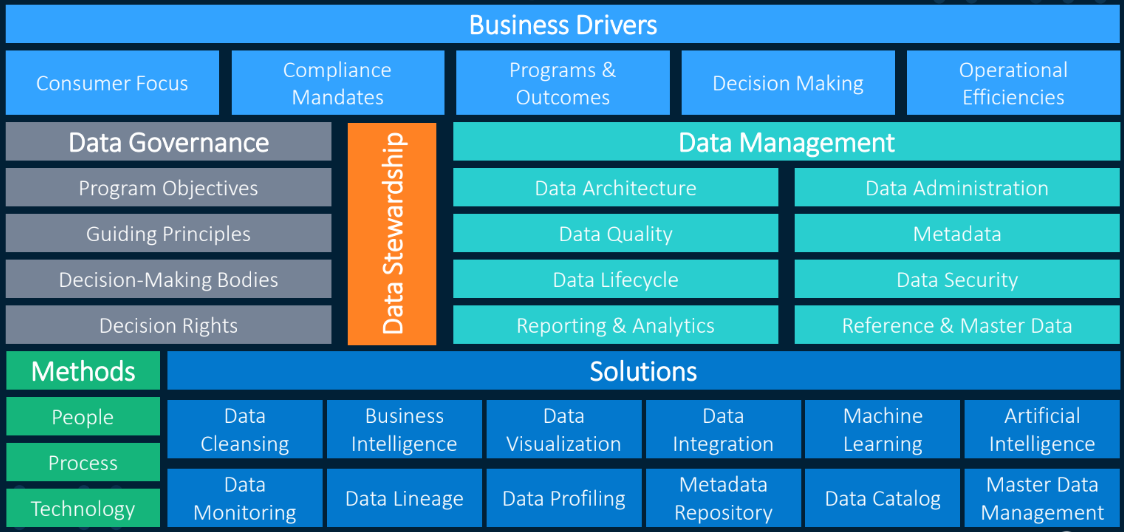
\includegraphics[scale=0.55]{images/SAS Data Management Framework.png}
    \caption{SAS Data Management Framework}
    \label{SAS DMF}
\end{figure}

SAS Data Management, as part of the SAS Data Management Framework, is a set of principles that cover policies and standards about data collection, storage, and processes. 

\begin{figure}[H]
\begin{center}
    \renewcommand{\arraystretch}{1.5}
    \begin{tabular}{|>{\raggedright\arraybackslash}m{3.5cm}
                    |>{\raggedright\arraybackslash}m{11.5cm}
                    |}
    \hline
    \rowcolor[HTML]{196fb4}\centering\textcolor{white}{\large Principle} 
                            & \centering\textcolor{white}{\large Description} 
                            \tabularnewline 
    \hline
    Data Architecture & Models, policies, rules, standards about what data is captured, how it is stored, arranged and integrated (data analysis, data modeling, data design). \\\hline
    Data Quality & Quality of data, its integrity and how its is cleansed and/or enriched. \\\hline
    Data Lifecycle & How data is created, stored, distributed, used, maintained, archived, and disposed. \\\hline
    Reporting & Analytics \& Systems that support the creation of value from data. \\\hline
    Data Administration & Day-to-day management and control of data and databases. \\\hline
    Metadata & Capture, storage, documentation, and publishing of information about enterprise data such as its description, lineage, usage, ownership, etc. \\\hline
    Data Security & How data is accessed and secured and how privacy is handled. \\\hline
    Reference \& Master Data & Correct and consistent management of master and reference data. \\\hline
    \end{tabular}
\end{center}
\caption{8 Principles of Data Management}
\label{8 DMA Principles}
\end{figure}

\begin{figure}[H]
    \centering
    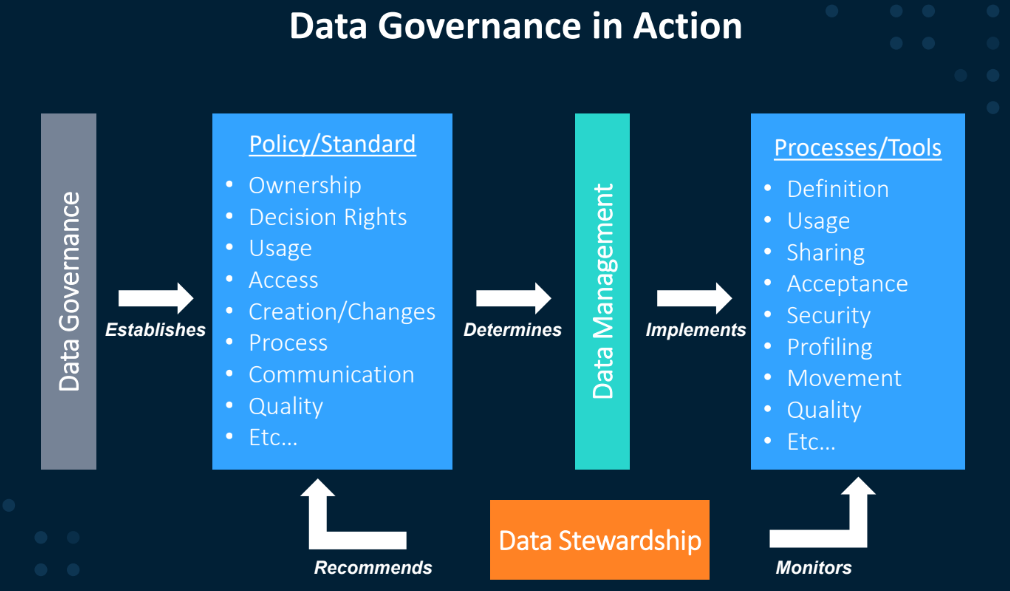
\includegraphics[scale=.60]{images/SAS Data Governance In Action.png}
    \caption{SAS Data Governance in Action}
    \label{SAS DGIA}
\end{figure}

Engaging in data governance without achieving data management outcomes is merely an academic exercise and is bound to fail. Similarly, conducting data management without proper data governance perpetuates a culture of reliance on unreliable sources and informal knowledge sharing. 

Data stewards play a vital role in actively monitoring data and advocating for organizational policies, serving as the vital link between data governance and data management activities.

\subsection{Data Stewardship}
A data steward is someone whose role is to develop and protect the information resources for the organization and ensures the integrity of the data. However, data stewardship is not data governance, it is a critical part of data governance. 

\begin{figure}[H]
\begin{center}
    \renewcommand{\arraystretch}{1.5}
    \begin{tabular}{|>{\raggedright\arraybackslash}m{4cm}
                    |>{\raggedright\arraybackslash}m{8cm}
                    |}
    \hline
    \rowcolor[HTML]{196fb4}\centering\textcolor{white}{\large Principle} 
                            & \centering\textcolor{white}{\large Description} 
                            \tabularnewline 
    \hline
    Metadata & Common definitions, Data dictionary, Data mining, Data lineage. \\\hline
    Data Quality & Continuous improvement, Root cause analysis, Measurement. \\\hline
    Architecture & Standards, Scalable solution(s). \\\hline
    Data Trust & Standards, Policies. \\\hline
    Data Integration & Transparent processes, Data ready for use. \\\hline
    People and Process & Teamwork, Facilitation, Consensus building. \\\hline
    Business Needs & Identify, Set priorities, Alignment of data with business needs. \\\hline
    Communication & Catalyst for change, Data evangelist.\\\hline
    \end{tabular}
\end{center}
\caption{8 Principles of Data Stewardship}
\label{Data Steward's Job}
\end{figure}

\subsection{Metadata}
Metadata can be defined as data about data, serving as valuable information that assists in navigating the intricate network of data within an organization and facilitates its effective utilization.

\subsubsection{Metadata Management}
The practice of gathering, storing, and provisioning information about data assets.

Metadata plays a crucial role in various aspects of data management and analytics within an organization. It serves to increase confidence in the data by providing valuable context and understanding. 

Operational efficiencies are harmonized as redundant data and processes are identified, streamlining operations. Effective communication between data creators, consumers, and IT is facilitated, fostering collaboration and alignment. This reduces the time to market by decreasing the development life cycle and enabling faster data research. Change management and impact analysis for IT become simpler, ensuring smooth transitions and minimizing disruptions. 

\subsubsection{Types of Metadata}
There are 3 types of metadata used by organizations.

\begin{figure}[H]
\begin{center}
    \renewcommand{\arraystretch}{1.5}
    \begin{tabular}{|>{\raggedright\arraybackslash}m{3.5cm}
                    |>{\raggedright\arraybackslash}m{3cm}
                    |>{\raggedright\arraybackslash}m{8cm}
                    |}
    \hline
    \rowcolor[HTML]{196fb4}\centering\textcolor{white}{\large Metadata Type} 
                            & \centering\textcolor{white}{\large Data Owner} 
                            & \centering\textcolor{white}{\large Metadata Objective} 
                            \tabularnewline 
    \hline
    Business Metadata & Business & Provide a road map to navigate in business context the complex network of data an organization has. \\\hline
    Technical Metadata & Technical & Technical characteristics of data used by IT staff to design efficient databases, queries, and applications and to reduce data duplication.\\\hline
    Operational Metadata & Technical & Describes characteristics of routine operations.\\\hline
    \end{tabular}
\end{center}
\caption{Types of Metadata}
\label{Types of Metadata}
\end{figure}

\begin{enumerate}
    \item Business Metadata Examples:
    \begin{itemize}
        \item Business name and description, data location, data usage, business rules, access instructions, valid range of values, relationship to other data elements, data owner and steward, and data security classification.
    \end{itemize}
    \item Technical Metadata Examples: 
    \begin{itemize}
        \item Table name, column name, data type, data size, primary and foreign key attributes, optionality, nullability, database server identifier, and data lineage.
    \end{itemize}
    \item Operational Metadata Examples:
    \begin{itemize}
        \item Schedules and batch jobs, logs of job execution, error logs, audit, balance, and control measures, SLA requirements, volume and usage statistics, backup and archival information, and daily ETL processes.
    \end{itemize}
\end{enumerate}

\begin{figure}[H]
    \centering
    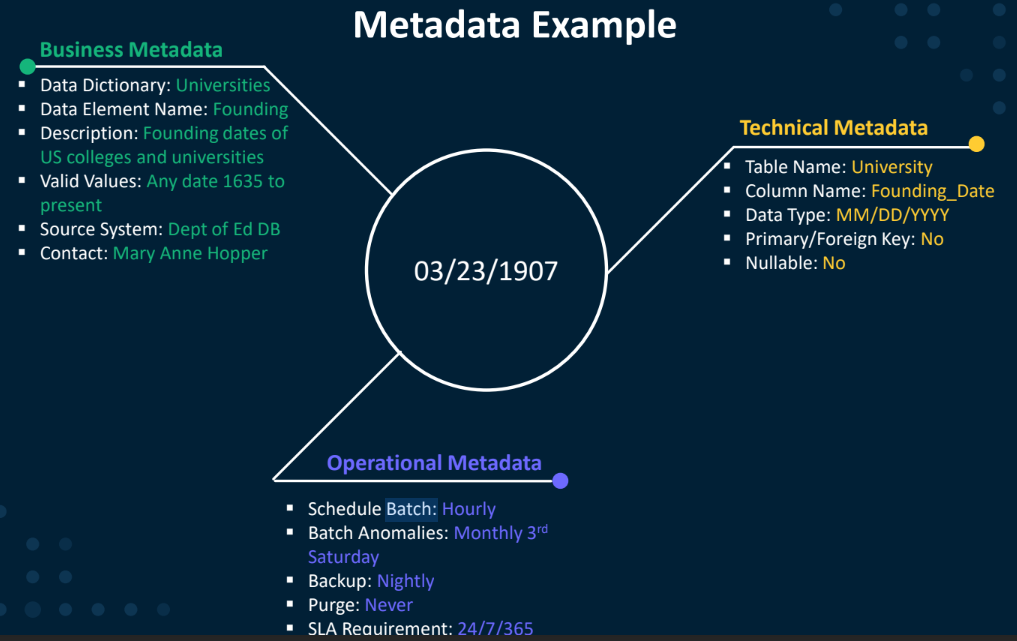
\includegraphics[scale=0.60]{images/Metadata Example.png}
    \caption{Example of Metadata}
    \label{Metadata Example}
\end{figure}

\subsubsection{Metadata Management Cycle}

\begin{figure}[H]
    \centering
    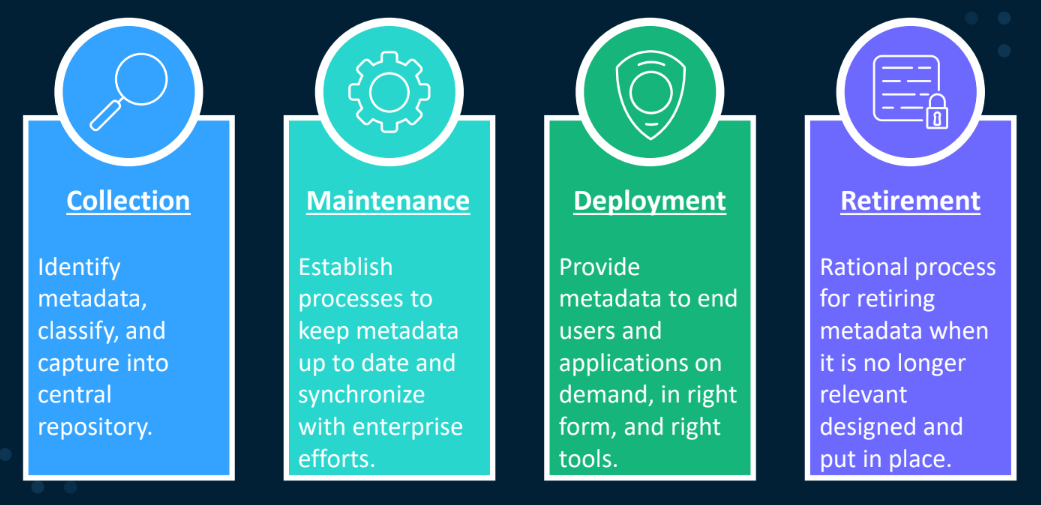
\includegraphics[scale=0.58]{images/Metadata Management Lifecycle.png}
    \caption{Metadata Management Lifecycle}
    \label{Metadata Management Lifecycle}
\end{figure}

\subsection{Data Dictionaries}
A data dictionary defines the structure and contents of data sets, databases, applications, or warehouses.

A recommended approach involves using a standardized document to create a proper dictionary that provides insights into the structure and contents of data sets, databases, applications, or warehouses. Developing a data dictionary requires access to the data, which may necessitate data sharing agreements such as business association agreements for HIPAA compliance. The data dictionary acts as a reference guide that defines the various aspects of data, aiding in its management and utilization. 

To begin building a data dictionary, it is recommended to start with organization critical metadata elements. 

\begin{figure}[H]
\begin{center}
    \renewcommand{\arraystretch}{1.5}
    \begin{tabular}{|>{\raggedright\arraybackslash}m{3.5cm}
                    |>{\raggedright\arraybackslash}m{11cm}
                    |}
    \hline
    \rowcolor[HTML]{196fb4}\centering\textcolor{white}{\large Data Dictionary} 
                            & \centering\textcolor{white}{\large Description}
                            \tabularnewline 
    \hline
    Data Element Name & Business name of element \\\hline
    Description & Business Description \\\hline
    Data Type & Physical data type (varies depending on database platform) \\\hline
    Valid Values & Valid data ranges; 1,0 for measures; valid date range \\\hline
    Source System & Source system database - may need to insert additional columns for multiple load stops (staging, DW $\rightarrow$ DM) \\\hline
    Contact & Data Owner or Data Steward contact person \\\hline
    \end{tabular}
\end{center}
\caption{Key Organization Critical Metadata Elements}
\label{Data Dictionary}
\end{figure}

%<---------------- second day ---------------->
\subsection{Data Quality}
Data quality is the conformance of data to the business definitions and the business rules (i.e., business metadata).

\subsubsection{Data as a True Asset}
Effective planning and management of data is essential, as it is a valuable and reusable asset that can increase in value through integration and analysis. Managing the quality of both data and metadata is crucial, requiring input from cross-functional teams with diverse skills and expertise. 

Data possesses unique properties, and its value can be expressed both qualitatively and quantitatively. Taking an enterprise-wide perspective is necessary to fully leverage the potential of data and maximize its value.

\subsubsection{Organizational Reasons for Poor Data Quality}
The lack of data stewardship and data governance, along with poor metadata management and absence of data lineage, contribute to misconceptions about data quality. 

Key data elements may not be clearly defined, and the emergence of new data sources outpaces effective management. Manual data entry without quality checks further hampers data integrity. Insufficient monitoring, reporting, and absence of defined service level agreements for essential business data quality exacerbate the issue. Moreover, the absence of clear data ownership and a culture that recognizes data as a valuable business asset perpetuate these data quality misconceptions.

\subsubsection{Data Quality Scope}
\begin{itemize}
    \item Business Definition Quality (\textit{Context})
    \begin{itemize}
        \item Business Definitions. Business Rules. Valid Content (valid values, range). Intended Business Purpose (correct usage context). Current Data Quality.
    \end{itemize}
    \item Data Record Quality (\textit{Rows})
    \begin{itemize}
        \item Item completion. Duplication. Cross-table validation. Accuracy.
    \end{itemize}
        \item Data Element Quality (\textit{Columns})
    \begin{itemize}
        \item Domain Integrity: Data type of field (ex. Date). Correct Contextual Value: Business metadata and business rule validation. Accuracy: Source system or expected calculation validation. Cross-Field Validation: Validates the business rule that relates two or more
        columns or across tables. Format Consistency: Correct format (ex. MM/DD/YYYY).
    \end{itemize}
    \item Data Movement Quality (\textit{Navigation})
    \begin{itemize}
        \item External data quality (incoming – outgoing). Source System to Source System (file transfer, SOA). Source System to data mart / data warehouse. Data Warehouse to Data Marts. To desktops via self-service data. Internal to Cloud – Cloud to Internal. 
    \end{itemize}
\end{itemize}

\subsection{Data Governance Journey}

\subsubsection{Plan: Identify organization needs, opportunities, and efforts}
During the planning phase, objectives of the program must be defined and frameworks must be set for how and when decisions will be made.

The planning phase must discuss the initial scope of data governance, objectives, guiding principles, organizational frameworks, roles, responsibilities, and the program charter.  

\subsubsection{Design: Who makes the decisions and how}
During the design phase, decision-making bodies will determine operating procedures and how
compliance and progress will be measured. Design methodologies should be decided by an official council of data stewards. 

A defined subset of rules should be established that are non-negotiable and must be strictly adhered to. The success of these rules lies in their ability to facilitate the progress of data stewardship, thereby generating tangible value. To validate the effectiveness of your plan, it is recommended to develop a program measurement plan.

This plan involves comparing the current state with previous meetings, using metrics such as steward attendance. For instance, evaluating decision-making based on a required quorum, such as 8 out of 10 members, ensures a robust decision-making process. Furthermore, it is important to note that proxies are not permissible, and the punctuality of members attending the meetings should also be monitored as part of the measurement plan.

A standardized solution to define key activities and assign decision making rights is through a RACI chart. 

\begin{figure}[H]
    \centering
    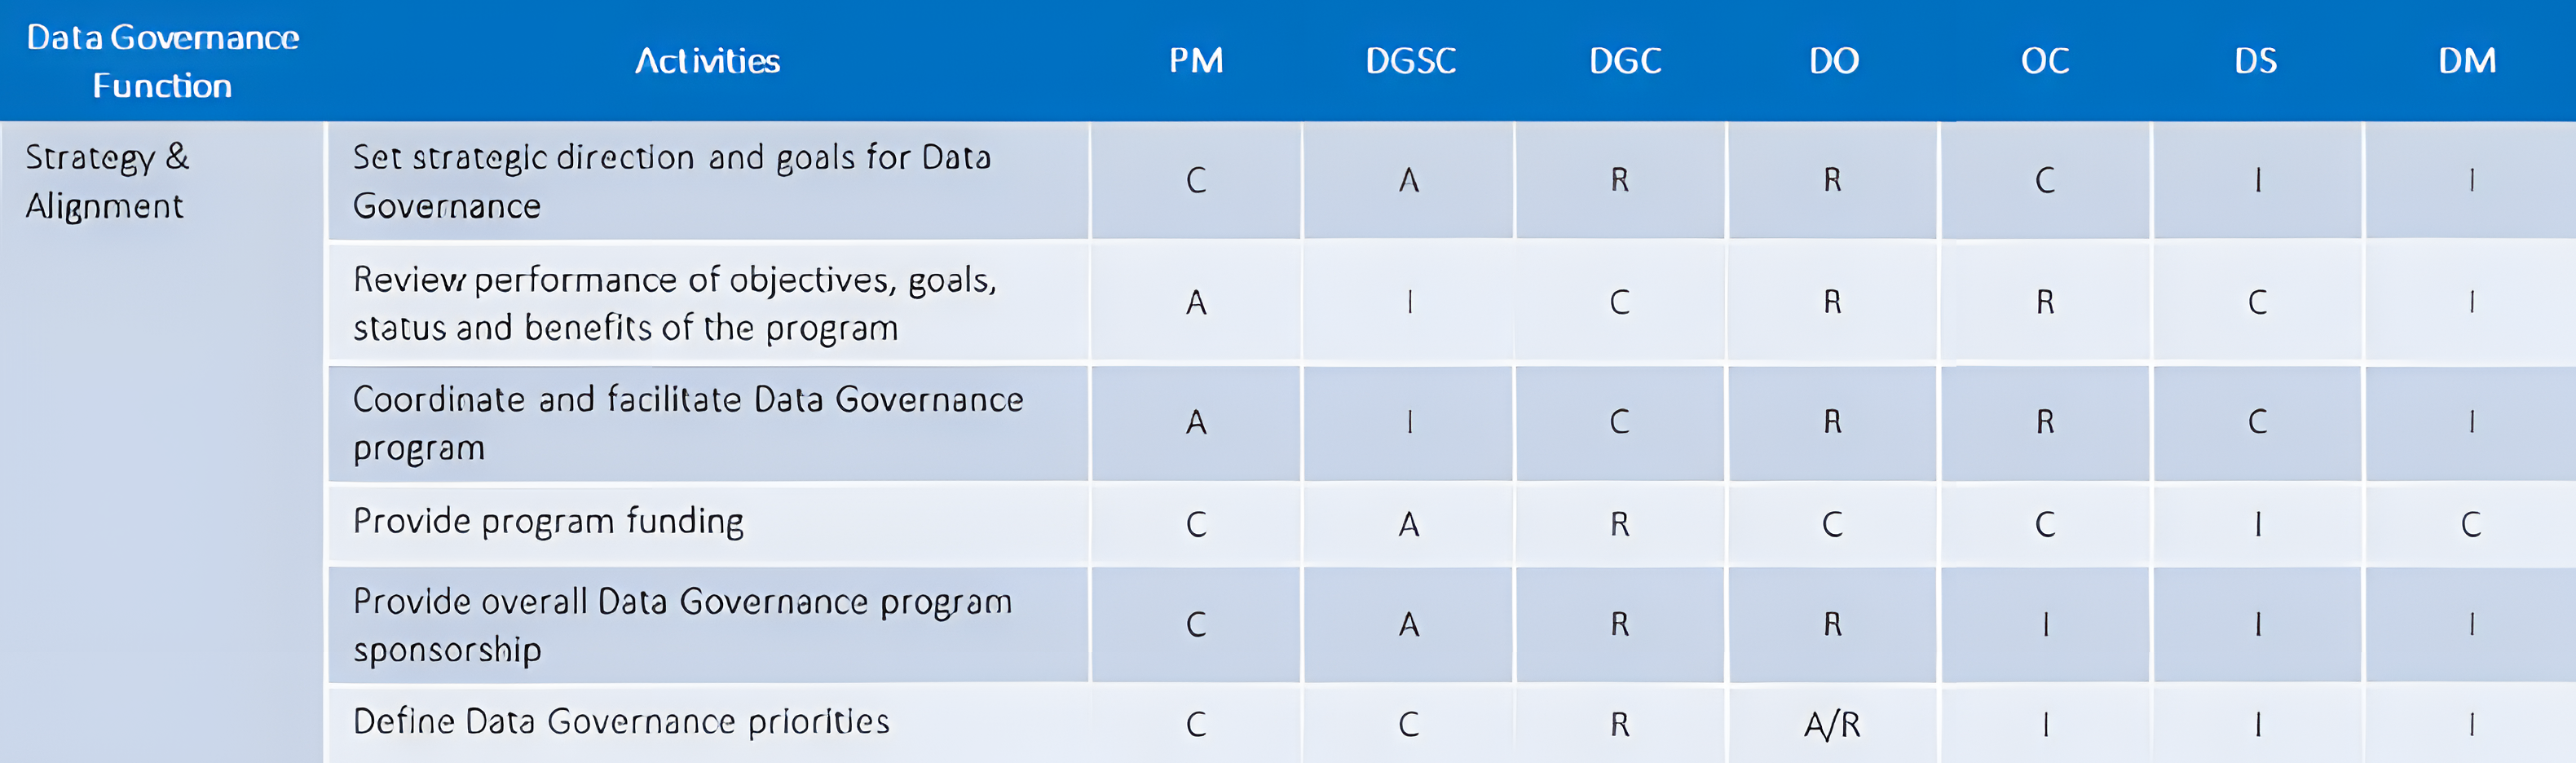
\includegraphics[scale=0.143]{images/RACI-example.png}
    \caption{A Sample RACI Chart \\ \textit{R} = Responsible, \textit{A} = Accountable, \textit{C} = Consulted, \textit{I} = Informed}
    \label{RACI-example}
\end{figure}

\subsubsection{Launch: Kick off initial program – begin small and expand}
During the launch phase, the designed operating model will be executed. 

\begin{enumerate}
    \item Onboard participants: Engage and onboard relevant stakeholders, ensuring their understanding of their roles and responsibilities within the project.
    \item Execute operating model: Implement the established operating model, which defines the framework and processes for data governance.
    \item Policy development and approval: Develop and finalize data governance policies, ensuring alignment with organizational objectives and obtaining necessary approvals.
    \item Benefit measurement: Establish a measurement plan to assess the effectiveness of the data governance. This involves defining metrics and tracking progress against predefined goals.
\end{enumerate}

\subsection{Policy}
A policy refers to a documented set of principles, guidelines, and rules that govern the management, access, usage, and protection of data within an organization. 

\begin{figure}[H]
\begin{center}
    \renewcommand{\arraystretch}{1.5}
    \begin{tabular}{|>{\raggedright\arraybackslash}m{3cm}
                    |>{\raggedright\arraybackslash}m{11.5cm}
                    |}
    \hline
    \rowcolor[HTML]{196fb4}\centering\textcolor{white}{\large Principle} 
                            & \centering\textcolor{white}{\large Description}
                            \tabularnewline 
    \hline
    Policy & Formal set of statements that define how data resources will be used or managed. \\\hline
    Procedure & Detailed instructions about how a policy is to be implemented.\\\hline
    Standard & Required configuration that is considered best practice. \\\hline
    Best Practice & Technique, method, process, or activity that is more effective at delivering a particular outcome than any other technique, method, process, etc. \\\hline
    Data Management & Tactical execution and enforcement of data governance policies and standards. \\\hline
    \end{tabular}
\end{center}
\caption{Principle Comparison Against Policy}
\label{Policy Comparison}
\end{figure}

\subsubsection{Policy Statement - Sample}
The Data Governance Office, in partnership with the appropriate organization entities and support from IT, will proactively assess, monitor, report, and improve data quality. For the purposes of this policy, data quality is defined as the conformance of data to the definitions and the organization rules (metadata).

\subsection{Additional: Questions \& Answers}

To ensure the conversation remains as relevant as possible to UHTASI, dedicated time slots were allocated for question and answer sessions. (Key: \textit{UHTS = UHTASI, SAS = SAS})

\begin{enumerate}
    \item UHTS $\rightarrow$ SAS: \textit{Is there a formal data strategy that outlines, access, integration, movement, storage?}
    \begin{itemize}
        \item \textit{The inherent issue is that not everything is harmonized across organizations, therefore, there is no unified organizational strategy that solves the problem. Instead, the one responsible for providing a solution that fits the organizational needs is the principle investigator.}
    \end{itemize}
    \item SAS $\rightarrow$ UHTS: \textit{How does UHTASI handle data validation?}
    \begin{itemize}
        \item UHTASI mainly uses hash check-sums in R and python for data validation. We hope that SAS software alleviate these, or lack-there-of, validation issues. UHTASI checks for missing cells and duplicates in data, however, these cases do not entirely indicate missing data values. Data sources are not standardized amongst our data providers. Therefore, ETL pipelines, data integration, and data quality are also not standardized.
    \end{itemize}
    \item SAS $\rightarrow$ UHTS: \textit{What are common problems that UHTASI's analysts are facing regarding data?}
    \begin{itemize}
        \item UHTASI's ETL process is dependent on the type of data source that is being used. In the case of federal government data, UHTASI will be provided be an encrypted drive with public/private key authentication processes. However, even a straight forward solution as above requires the tracking an auditing of actions throughout the ETL process. 
        \item UHTASI has difficulty getting access to timely data. Data is provided quarterly by vendors and general trust are established across each vendor.
    \end{itemize}
\end{enumerate}

% < ------- third day ----------->
\newpage
%What are we installing?
\begin{itemize}
    \item SAS 9
    \begin{itemize}
        \item Base SAS
        \item Data Management Advanced Server
        \begin{itemize}
            \item Data Governance - DG Lineage, DDG Workflow, 
            \item Data Integration Studio - High/Enterprise level data access, integration, and management using visual flow charts. (Flow charts are converted to SAS code). More for IT/Admin.
            \item Data Quality - Helps standardize data, duplicate records, errors using visual flow charts and built in (out-of-box) algorithms. (Flow charts are converted to SAS code). More for "everybody". Meant to integrate with other software smoothly because data quality should be checked throughout the entire ETL process. 
            \item Enterprise Guide - Low/Mid data management and access using visual flow charts. (Flow charts are converted to SAS code). More for "everybody".
        \end{itemize}
        \item SAS/ACCESS to MS
    \end{itemize}
    \item SAS Viya
    \begin{itemize}
        \item Viya Platform
        \item Visual Analytics
        \item Visual Statistics
        \item Visual Data Mining and ML
        \item Visual Text Analytics
        \item Visual Forecasting
        \item Model Manager
        % Software below will not be covered but is installed.
        \item SAS Optimization
        \item SAS IML
        \item SAS QC
        \item SAS Econometrics
        \item Data Preparation 
        \item SAS/ACCESS Engines
        \item Visual Analytics Add-In For Office 
    \end{itemize}
\end{itemize}

% <------------ additional questions ----------->
\newpage

%Creates the Massively Learning Activities section.
\section{Massively Learning Activities} \label{section: MLA}
\begin{itemize}
    \item \textcolor{red}{We are contracted by CNMI to create an infrastructure where we can perform data analytics on PHI. This infrastructure is hosted on-prem first, hybrid later.}
    \item \textcolor{red}{Tenants (e.g. APCD, CMNI, CMA, Criminal Justice) has the data ready.}
    \item \textcolor{red}{Data is submitted from tenants to ETL (data-pipeline) to be processed then sent to SAS (on-prem servers).}
    \item \textcolor{red}{Data analytics is performed on the data using advanced algorithms in SAS programming language}. 
    \item \textcolor{red}{Project is time sensitive, deadline is requiring TASI to move onto the development stage with existing on-prem hardware as proof-of-concept ASAP}.
    \item \textcolor{red}{Initially architect the infrastructure using existing on-prem hardware to speed up deployment}
    \item \textcolor{red}{Once deployed, stable, and proof-of-concept ready, move onto the production stage by acquiring new hardware and migrating the previous (virtualized) SAS deployment to the new hardware using vMotion.}.
    \item \textcolor{red}{Configure the security relationship between the software, hardware, and tenants (Active Directory, LDAP, Security Groups, etc}.
\end{itemize}

The System Development Lifecycle (SDLC) is a project management model that defines different stages that are necessary to bring a project from conception to deployment and later maintenance. Massively Learning Activities will follow a similar variation to the SDLC project management model where each SDLC stage corresponds to a subsection in this chapter. 

\subsection{Planning Stage}
Massively Learning Activities (MLA) is divided into two phases, (1) the initial deployment of SAS on existing infrastructure and later (2) the migration of SAS onto scaled infrastructure. 

In either deployment stage, SAS Viya will be deployed in a multi-tenant environment. A multi-tenant deployment of SAS Viya allows for a single deployment to serve multiple customers\footnote{Customers are tenants (etc: CNMI, APCD, CMA, Med-Quest, UH Education) but each tenant has its own set of users and groups.}. These customers can share some physical resources while remaining logically separated. A multi-tenant deployment allows for these distinct groups to share IT resources in a secure and cost-effect manner. Multi-tenancy deploys into a \href{https://kubernetes.io/}{Kubernetes} namespace. The deployment includes a provider tenant, shared mid-tier services, application-specific database schemas, shared applications, and a designated SAS administrator for the provider tenant. Administrators with elevated Kubernetes privileges onboard one or more tenants. After tenant on-boarding, Kubernetes administrators onboard one or more Cloud Analytic Services into each new tenant, then each CAS server is uniquely configured during the on-boarding process to meet the specific tenant requirements. 

The final and completed deployment of SAS Viya will expect a total of 8 tenants:

\begin{itemize}
    \item \textbf{Tenant 1}: Commonwealth of the Northern Mariana Islands (CNMI)
    \item \textbf{Tenant 2}: All-Payer Claims Database (APCD)
    \item \textbf{Tenant 3}: Centers for Medicare \& Medicaid Services (CMA)
    \item \textbf{Tenant 4}: Med-Quest
    \item \textbf{Tenant 5}: UH Education 1
    \item \textbf{Tenant 6}: UH Education 2
    \item \textbf{Tenant 7}: UH Education 3
    \item \textbf{Tenant 8}: UH Education 4
\end{itemize}

%\textcolor{red}{\lipsum[1-1]}

MLA is a time sensitive project that requires deployment of SAS Viya in a multi-tenant environment as soon as possible. Therefore, an initial deployment of SAS Viya and SAS DMA will be conducted on existing on-premise infrastructure with only half the amount of tenants by \textcolor{red}{Q4 2023}. 

\subsubsection{Initial Deployment}
The initial deployment of MLA will involve installing SAS on existing infrastructure\footnote{Infrastructure is used to describe existing hardware available to use on-premises at TASI/PHIDC.}. The existing infrastructure is  an available Dell PowerEdge FX2 Enclosure located in TASI's NOC. The PowerEdge FX2 Enclosure is a 2U hybrid rack-based computing platform that combines multiple blades\footnote{Blades are complete servers in a smaller form factor that have their own CPU(s), memory, storage, and networking components.} into a single enclosure to increase the efficiency of, and reduce the cost of, rack-based systems. This multi-blade enclosure has a \textcolor{red}{fill me GB} connection to a \textcolor{red}{storage pool (describe me)}.

\begin{figure}[H]
    \centering
    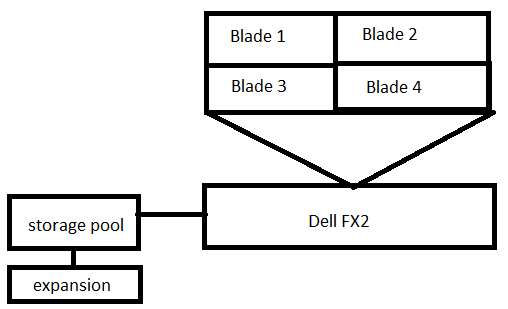
\includegraphics[scale = 0.5]{images/currentENV.png}
    \caption{TASI On-Premise Environment \textcolor{red}{(needs VISIO)} }
    \label{Current ENV}
\end{figure}

It is important to note that each blade in the FX2 chassis is already in use by other TASI projects. Therefore, the multi-tenant SAS architecture will be logically separated based on the available resources within each blade. Each blade is equipped with \textcolor{red}{[core count]} CPU, \textcolor{red}{[memory count]} RAM, and \textcolor{red}{[size]} storage. 

This deployment will have CNMI, APCD, CMA, and Med-Quest as the initial four tenants and each tenant will have a different deployment configuration based on their requirements. As of \textcolor{red}{March 3, 2023}, CNMI and APDC will be configured in a 5-server environment \footnote{5 Server: (1) Primary CAS Controller, (2) Backup CAS Controller, (3) CAS Worker 1, (4) CAS Worker 2, (5) CAS Worker 3} and every other tenant will be configured in a 3-server environment\footnote{3 Server: (1) Primary CAS Controller, (2) Backup CAS Controller, (3) CAS Worker 1}. The other tenants that are yet to be added will be considered during the migration stage of MLA. 

\begin{figure}[H]
    \centering
    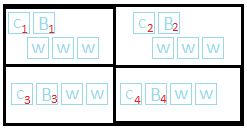
\includegraphics[scale = 1]{images/sas-initial-deployment.png}
    \caption{SAS Initial Deployment \textcolor{red}{(needs VISIO)} }
    \label{SAS Initial Deployment}
\end{figure}


\subsubsection{Migration Deployment}
\textcolor{red}{\lipsum[1-1]}

\subsection{Requirements of Analysis Stage (Sizing)}
\textcolor{red}{Refer to the sizing documents (2) and the current resources document comparison to see what we are missing.}


\subsection{Design and Prototyping Stage}

\subsection{Initial Development Stage}

\subsection{Testing Stage}

\subsection{Implementation and Integration Stage}

\subsection{Migration Stage (SDLC II)}

\subsection{Operations and Maintenance Stage}

\subsection{End-Game Implementation}
\textcolor{red}{environmental scan for the future environment}
\newpage

%Creates the HCI section. 
\section{Hyper-Converged Infrastructure (HCI)} \label{section: HCI}

HCI, or Hyper-Converged Infrastructure, is a software-defined, unified system that combines the traditional elements of IT infrastructure (e.g., compute, networking, management, storage) with virtualization, simplifying infrastructure, reducing costs, and increasing scalability and flexibility. In a traditional IT Infrastructure, servers, storage networks, and storage systems are physically separated as stand alone hardware devices (e.g., servers, network switches, disk arrays). Consolidating these components into a single, integrated system simplifies the management, deployment, configuration, and maintenance of your IT Infrastructure. 

The benefits of an HCI environment include: 
\begin{itemize}
    \item Scalability: Designed to scale out by adding additional nodes on-demand to your system.
    \item Efficiency: Improve resource utilization by using or eliminating idle storage capacity.
    \item Agility: Quickly deploy new applications and workloads without extensive planning across systems. 
    \item Data Protection: Integrated backup and disaster recovery.
    \item Reduced Hardware Costs: Reduce the amount of hardware required reducing CAPEX\footnote{Capital expenditure is the cost a business incurs to acquire assets that will provide benefits beyond the current year.}/OPEX\footnote{Operating expenses refer to the money a company spends to run day-to-day operations.} costs. 
\end{itemize}

% Single-Machine HCI Relationship with Cloud Deployments %
%\begin{figure}[H]
%    \centering
%    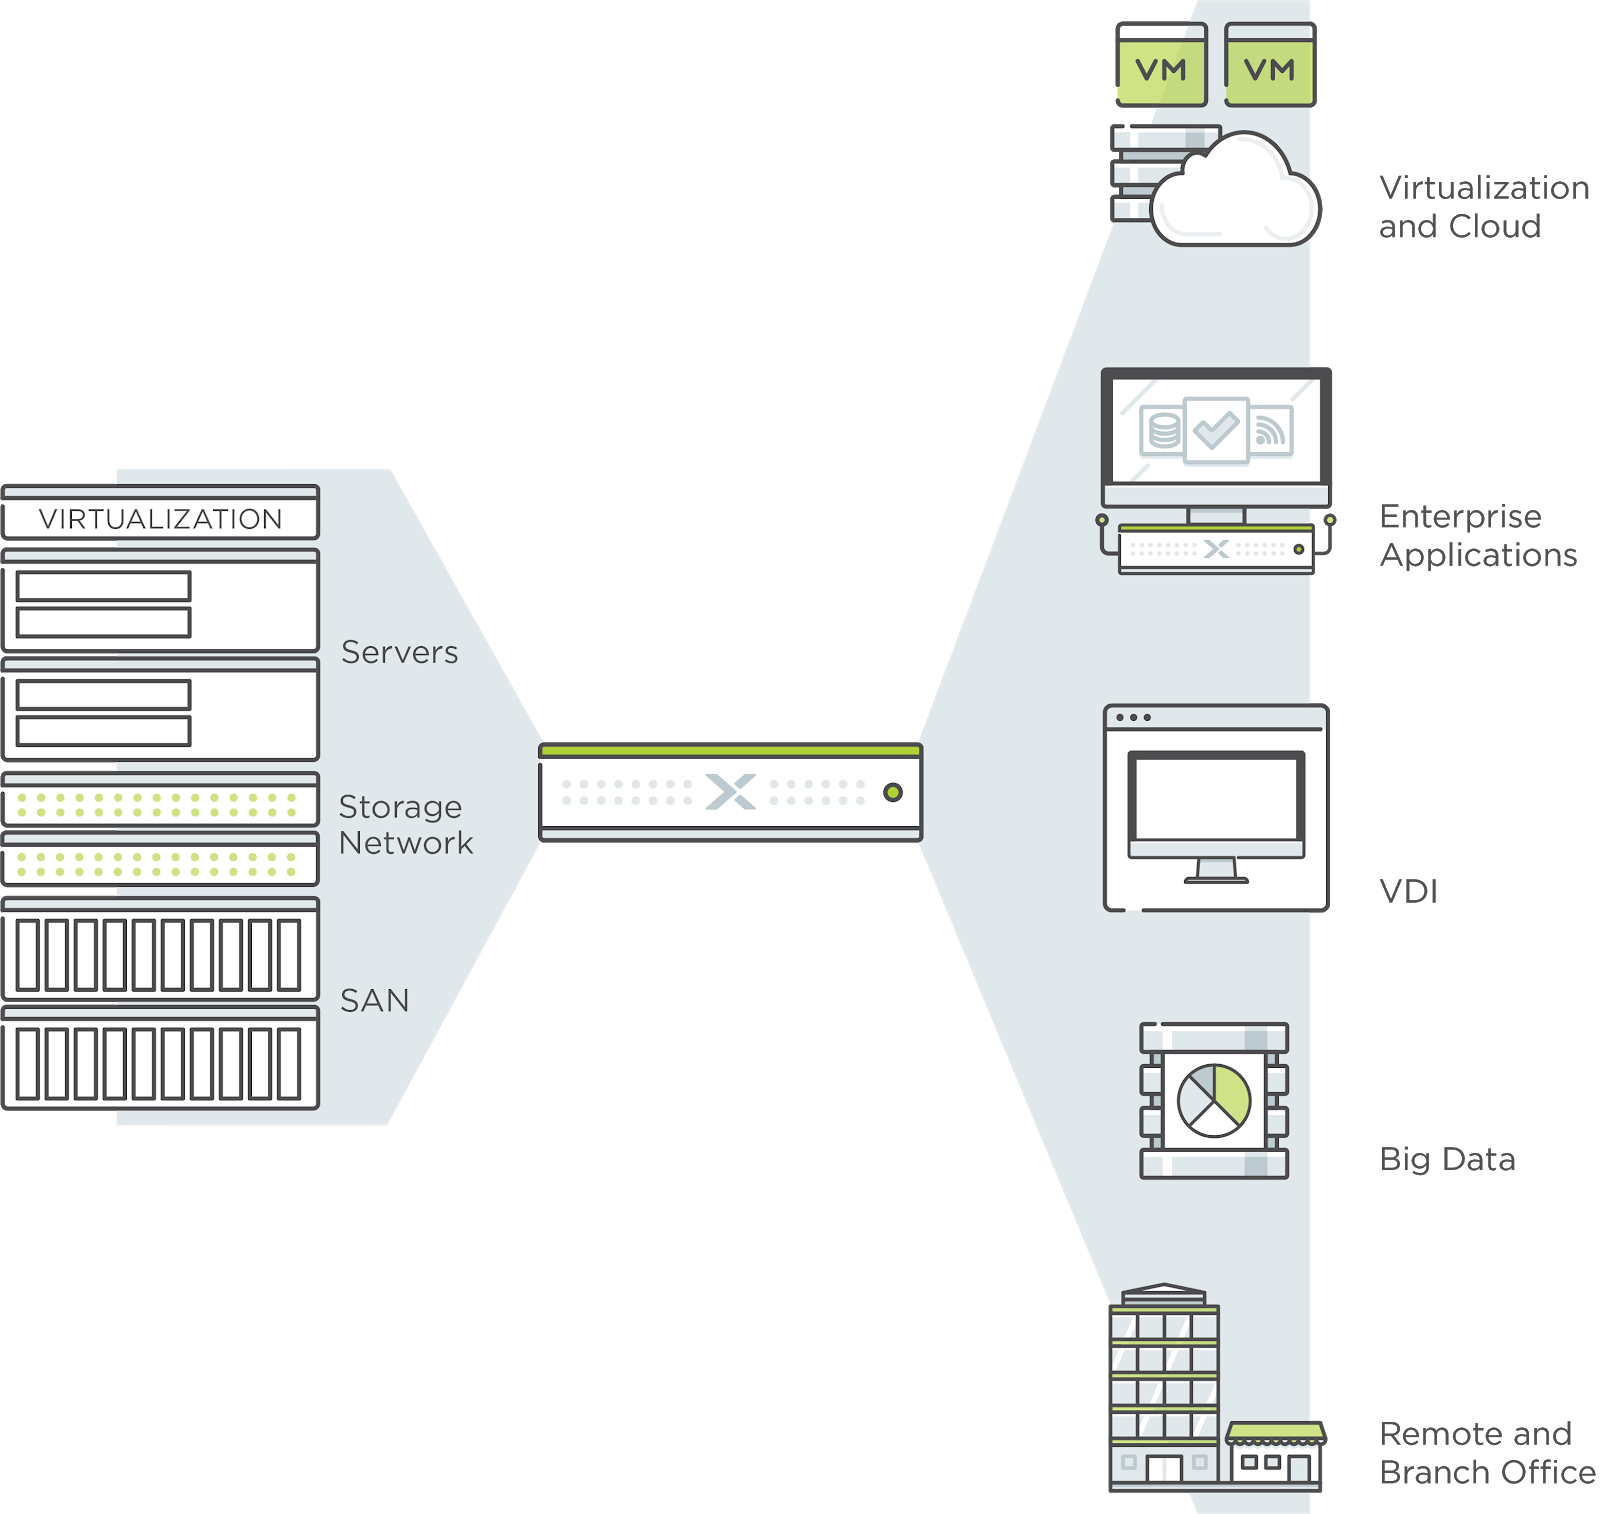
\includegraphics[scale = 0.25]{images/HCI_Nutanix_Node.png}
%    \caption{Single-Machine HCI \textcolor{red}{(STOLEN EXAMPLE)}}
%    \label{HCI Explained (Single-Machine)}
%\end{figure}

\begin{figure}[H]
    \centering
    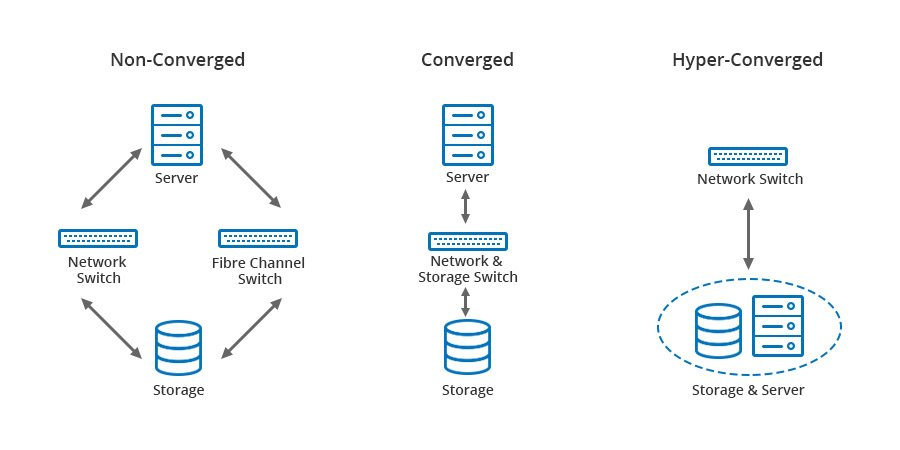
\includegraphics[scale = 0.5]{images/HCI_tldr.jpg}
    \caption{\href{https://en.wikipedia.org/wiki/Hyper-converged_infrastructure}{Types of IT Infrastructures}}
    \label{HCI Convergance Comparison}
\end{figure}

In HCI, multiple servers or nodes are combined to create a cluster. These nodes share their computing and storage resources with each other to create a multi-purpose integrated system. The design of your HCI cluster will depend on your specific needs and requirements.

The software that powers HCI also includes a management layer, which automates tasks like resource provisioning, data migration, and load balancing. This layer abstracts the hardware, making it easier to manage and deploy your IT infrastructure. Overall, HCI is a powerful and flexible solution that can help organizations streamline their IT operations, reduce costs, and improve efficiency.


\newpage

%Creates the Massively Learning Activities section.
\section{Massively Learning Activities II - Migration Deployment} \label{section: MLA2}
TASI has been contracted by CNMI to create an infrastructure that allows for data analytics on Protected Health Information (PHI). This infrastructure will initially be hosted on-premises, with plans to move towards a hybrid solution in the future. To achieve this, we will be providing a Platform as a Service (PaaS) solution, by hosting SAS Viya services on our own hardware and allowing tenants to access and utilize the platform for their own analytics applications.

The tenants, including APCD, CMNI, CMA, Criminal Justice, and several Education environments, will provide the necessary data, which will be submitted to an ETL data pipeline for processing before being sent to SAS on-prem servers. Once the data has been processed, tenants may perform data analytics using advanced algorithms in SAS programming language.

To ensure secure operations, we will configure the security relationships between the software, hardware, and tenants using LDAP, security groups, encryption  and other related tools. Our goal is to architect a high-performance infrastructure that allows for advanced data analytics while maintaining the confidentiality and security of PHI.

Due to SAS being a time sensitive project, the initial deployment will have SAS suites and VMs installed on existing hardware, with plans to migrate the infrastructure to newly acquired hardware in the future.

\subsection{Planning}

The System Development Lifecycle (SDLC) is a project management model that defines different stages that are necessary to bring a project from conception to deployment and later maintenance. The SDLC model consists of several phases, which typically include requirements gathering, design, development, testing, deployment, and maintenance. The specific activities within each phase may vary depending on the project and the organization, but the basic principles are the same. The SDLC model is a flexible framework that can be adapted to suit the needs of different projects and organizations. It provides a systematic approach to software development that helps ensure that software is built efficiently, effectively, and with minimal risk.

Massively Learning Activities will follow a similar variation to the SDLC project management model where each SDLC stage will correspond to a subsection in this chapter. 

\subsection{Requirements of Analysis}
\textcolor{red}{Refer to the sizing documents (2) and the current resources document comparison to see what we are missing.}

\subsection{Security and Risks}
\textbf{Security In-Depth}
\begin{itemize}
    \item LDAP
    \item VMware Security Policies
    \item SAS Security Policies
    \item HIPPA, other Federal Laws
\end{itemize}

\subsection{Deployment and Prototyping II (Migration)}

\textcolor{red}{VMotion in action (See 6.1.2).}

\subsection{Testing \& Integration II}

\subsection{Operations and Maintenance II}


\newpage

% Copy this to add more chapters
%\section{Copy me} \label{section: copy me}
\lipsum[1-8]
%\newpage

% Creates references using the Biblatex 
%\bibliographystyle{plain}
%\bibliography{General/References.bib}
%\newpage

\appendix % Any section after this command will have a letter as an index

% Adds an appendix entry
\section{Appendix A title} \label{section: appendix A title}
\lipsum[1-8]
\newpage

\end{document}
